%\documentclass[anon,12pt]{colt2018} % Anonymized submission
\documentclass[final, 12pt]{colt2018} % Include author names

% The following packages will be automatically loaded:
% amsmath, amssymb, natbib, graphicx, url, algorithm2e

\title[More Adaptive Algorithms for Adversarial Bandits]{More Adaptive Algorithms for Adversarial Bandits}
\usepackage{float}
%\restylefloat{table}

\usepackage{algorithm}
\usepackage{times}
\usepackage{makecell}
\usepackage[final]{showlabels}
%\usepackage{tablefootnote}
\usepackage{threeparttable}
\allowdisplaybreaks
%\usepackage[ruled]{algorithm2e}
 %vlined, ,linesnumbered
\usepackage{bbm}
\usepackage{enumerate}
%\usepackage{amsmath,amsthm,amsfonts,amssymb,mathrsfs}
%\addbibresource{main.bib}
\newcommand{\p}{\prime}
\DeclareMathOperator*{\argmin}{argmin}
\DeclareMathOperator*{\argmax}{argmax}
\newcommand{\inner}[1]{ \left\langle {#1} \right\rangle }
\newcommand{\inn}[1]{ \langle {#1} \rangle }
\newcommand{\absolute}[1]{ \left\lvert {#1} \right\rvert }
\newcommand{\abs}[1]{ \lvert {#1} \rvert }
\usepackage{amsmath}
\newcommand\norm[1]{\left\lVert#1\right\rVert}
\newcommand{\reg}{\text{\rm Reg}}
%\newtheorem{lemma}{Lemma}
%\newtheorem{theorem}{Theorem}
\newtheorem{cor}[theorem]{Corollary}
%\newtheorem{remark}[theorem]{Remark}
%\newtheorem{remark}{Remark}
%\newtheorem{prop}{Proposition}
%\newtheorem{definition}{Definition}
%\newtheorem{assumption}{Assumption}
 % Use \Name{Author Name} to specify the name.
 % If the surname contains spaces, enclose the surname
 % in braces, e.g. \Name{John {Smith Jones}} similarly
 % if the name has a "von" part, e.g \Name{Jane {de Winter}}.
 % If the first letter in the forenames is a diacritic
 % enclose the diacritic in braces, e.g. \Name{{\'E}louise Smith}

 % Two authors with the same address
  % \coltauthor{\Name{Author Name1} \Email{abc@sample.com}\and
  %  \Name{Author Name2} \Email{xyz@sample.com}\\
  %  \addr Address}

 % Three or more authors with the same address:
 % \coltauthor{\Name{Author Name1} \Email{an1@sample.com}\\
 %  \Name{Author Name2} \Email{an2@sample.com}\\
 %  \Name{Author Name3} \Email{an3@sample.com}\\
 %  \addr Address}


 % Authors with different addresses:
 \coltauthor{\Name{Chen-Yu Wei} \Email{chenyu.wei@usc.edu} \\
 \addr University of Southern California
 \AND
 \Name{Haipeng Luo} \Email{haipengl@usc.edu}\\
 \addr University of Southern California
 }

\begin{document}

\maketitle

\begin{abstract}
We present preconditioned stochastic gradient descent (SGD) algorithms for the $\ell_1$ minimization problem $\min_{\xx}\|\AA \xx - \bb\|_1$ in the overdetermined case, where there are far more constraints than variables. Specifically, we have $\AA \in \R^{n \times d}$ for $n \gg d$. Commonly known as the Least Absolute Deviations problem, $\ell_1$ regression can be used to solve many important combinatorial problems, such as minimum cut and shortest path. SGD-based algorithms are appealing for their simplicity and practical efficiency.
% Our algorithms precondition the matrix $\AA$ and then solve the problem for the resulting matrix $\tilde{\AA}$ using gradient descent techniques.
Our primary insight is that careful preprocessing can yield preconditioned matrices $\tilde{\AA}$ with strong properties (besides good condition number and low-dimension) that allow for faster convergence of gradient descent. In particular, we precondition using Lewis weights to obtain an isotropic matrix with fewer rows and strong upper bounds on all row norms. We leverage these conditions to find a good initialization, which we use along with recent smoothing reductions and accelerated stochastic gradient descent algorithms to achieve $\epsilon$ relative error in $\Otil(nnz(\AA) + d^{2.5} \epsilon^{-2})$ time with high probability, where $nnz(\AA)$ is the number of non-zeros in $\AA$. This improves over the previous best result using gradient descent for $\ell_1$ regression. We also match the best known running times for interior point methods in several settings.

Finally, we also show that if our original matrix $\AA$ is approximately isotropic and the row norms are approximately equal, we can give an algorithm that avoids using fast matrix multiplication and obtains a running time of $\Otil(nnz(\AA) + s d^{1.5}\epsilon^{-2} + d^2\epsilon^{-2})$, where $s$ is the maximum number of non-zeros in a row of $\AA$. In this setting, we beat the best interior point methods for certain parameter regimes.


%We consider the $\ell_1$ minimization problem $\min_{\xx}||\AA \xx - \bb||_1$ in the overconstrained case, where there are far more constraints than variables. More specifically, we have $\AA \in \R^{n \times d}$ for $n \gg d$. By using Lewis Weights preconditioning on $\AA$ and a careful initialization, we show that a standard stochastic gradient descent algorithm achieves $\epsilon$ relative error in about $nnz(\AA) +  d^3\epsilon^{-2}$ time with high probability. If we leverage smoothing reductions in \cite{AllenZhuH16} and the accelerated stochastic gradient descent algorithms in \cite{AllenZhu17}, we can achieve a running time of about $nnz(\AA) + d^{2.5}\epsilon^{-2}$ with the same guarantees. Both of these running times improve over the previous results in \cite{YangCRM16} and the latter result is comparable to the best known running times for interior point methods \cite{LeeS15}.
%
%The key idea will be to use our preconditioning to restrict our consideration to matrices $\AA$ such that $\AA^T\AA = \II$ and every row norm of $\AA$ is upper bounded by $O(\sqrt{d/n})$. \cite{cohenpeng} show that sampling $\AA$ with Lewis weights takes about $nnz(\AA) +d^{\omega}$ time and approximately preserves the minimization problem. Moreover, we can assume $n\le O(d\epsilon^{-2}\log n)$ for the sampled matrix. We then prove that all leverage scores of the sampled matrix are approximately equal. Since rotations preserve leverage scores, we can then rotate our sampled matrix to ensure that our desired properties are met in about $d^{\omega}\epsilon^{-2}$ time.
%
%Finally, we also show that if our original matrix $\AA$ is such that $\AA^T\AA \approx \II$ and the row norms of $\AA$ are bounded, we can avoid using fast matrix multiplication and prove a running time of about $nnz(\AA) + s d^{1.5}\epsilon^{-2}$, where $s$ is the maximum number of non-zeros in a row of $\AA$.

%Consequently, we will be able to restrict our consideration to matrices $A$ such that $A^TA \approx I$, and all row norms are equal, which is to say $||A_{i,:}||_2 = \sqrt{\frac{d}{n}}$ for all $i$.
%
%With a careful choice of our initial $x$, we show that standard gradient descent and stochastic gradient descent algorithms under these further assumptions only require $O(\frac{d}{\epsilon^2})$ and $O(\frac{d^2}{\epsilon^2})$ iterations, respectively, to achieve $\epsilon$ relative error with respect to the minimum objective value. Accordingly, these methods each achieve respective total runtime of $O(\frac{md}{\epsilon^2})$ and $O(\frac{d^3}{\epsilon^2})$, along with an $O(m)$ preconditioning cost, improving over the previous results in \cite{MahoneySGD}.
%
%We further examine the consequences of our assumptions when combined with smoothing reductions in [cite] and accelerated gradient descent techniques in [cite,cite]. As a result we are able to further improve the running times to $O(\frac{md}{\epsilon})$ and $O(dn\log{1/\epsilon} + \frac{d^2\sqrt{n}}{\epsilon})$.
%
%Random sampling $d\epsilon^{-2}\log{d}$ rows of $A$ will only incur error $\epsilon$ and reduces the latter running time to $O(\frac{d^{2.5}\log{d}}{\epsilon^2})$, which is then comparable to interior point methods of [cite]

\end{abstract}

\begin{keywords}
multi-armed bandit, semi-bandit, adaptive regret bounds, optimistic online mirror descent, increasing learning rate
\end{keywords}

\section{Introduction}
% !TeX root = main.tex
\section{Introduction}
\label{sec:intro}
Generative models are often trained in an unsupervised fashion, fitting a model $q$ to a set of observed data $x_P \subseteq X$ drawn iid from some true distribution $p$ on $x\in X$. Now, of course $p$ may not exactly belong to family $Q$ of probability distributions being fit, whether $Q$ consists of Gaussians mixture models, Markov models, or even neural networks of bounded size. We first discuss the limitations of generative modeling without feedback, and then discuss our model and results.

%\subsection{Limitations of Generative Modeling from Positive Examples Alone}
Consider fitting a generative model on a text corpus consisting partly of poetry written by four-year-olds and partly of mathematical publications from the {\em Annals of Mathematics}. Suppose that learning to generate a poem that looks like it was written by a child was easier than learning to generate a novel mathematical article with a correct, nontrivial statement. If the generative model pays a high price for generating unrealistic examples, then it may be better off learning to generate children's poetry than mathematical publications. However, without negative feedback, it may be difficult for a neural network or any other model to know that the mathematical articles it is generating are stylistically similar to the mathematical publications but do not contain valid proofs.\footnote{This is excluding clearly fake articles published without proper review in lower-tier venues \citep{LabbeL13}.} 

As a simpler example, the classic Markovian ``trigram model'' of natural language assigns each word a fixed probability conditioned only on the previous two words. Prior to recent advances in deep learning, for decades the trigram model and its variant were the workhorses of language modeling, assigning much greater likelihood to natural language corpora than numerous linguistically motivated grammars and other attempts \citep{Rosenfeld00}. However, text sampled from a trigram is typically nonsensical, e.g., the following text was randomly generated from a trigram model fit on a corpus of text from the Wall Street Journal \citep{JurafskyM09}:
\begin{quote}
They also point to ninety nine point six billion dollars from two hundred
four oh six three percent of the rates of interest stores as Mexico and
gram Brazil on market conditions. 
\end{quote}

In some applications, like text compression using a language model \citep{WittenNC87}, maximizing likelihood is equivalent to optimizing compression. However, in many  applications involving generation, such nonsense is costly and unacceptable. Now, of course it is possible to always generate valid data by returning random training examples, but this is simply overfitting and not learning. Alternatively, one could incorporate human-in-the-loop feedback such as through crowdsourcing, into the generative model to determine what is a valid, plausible sentence.

In some domains, validity could be determined automatically. Consider a Markovian model of a well-defined concept such as mathematical formulas that compile in \LaTeX{}. Now, consider a $n$-gram Markovian character model which the probability of each subsequent character is determined by the previous $n$ characters. For instance, the expression \$\{2+\{x-y\}\$ is invalid in \LaTeX{} due to mismatched braces. For this problem, a \LaTeX{} compiler may serve as a validity oracle. Various $n$-gram models can be fit which only generate valid formulas. To address mismatched braces, for example, one such model would ensure that it always closed braces within $n$ characters of opening, and had no nested braces. While an $n$-gram model will not perfectly model the true distribution over valid \LaTeX{} formulas, for certain generative purposes one may prefer an $n$-gram model that generates valid formulas over one that assigns greater likelihood to the training data but generates invalid formulas. 

Figure \ref{fig:rectangle} illustrates a simple case of learning a rectangle model for data which is not uniform over a rectangle. A maximum likelihood model would necessarily be the smallest rectangle containing all the data, but most examples generated from this distribution may be invalid. Instead a smaller rectangle, as illustrated in the figure, may be desired.

\begin{figure}[h]\label{fig:rectangle}
\centering
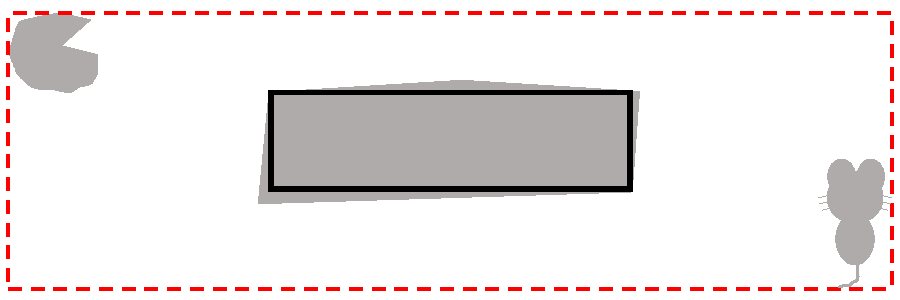
\includegraphics[width=3in]{fig.pdf}
\caption{Example where the underlying distribution $p$ is uniform over the (gray) valid regions. The solid rectangle maximizes our objective since it does not output nonsense (is supported only within the grey matter) and is closest to the $p$ (covers the maximum amount of grey matter). In contrast, the standard maximum likelihood (dashed red) rectangle must fully contain the observed samples, thus generating invalid points most of the time.  }
\end{figure}

Motivated by these observations, we evaluate a generative model $q$ on two axes. First is {\em coverage}, which is related to the probability assigned to future examples drawn from the true distribution $p$. Second is {\em validity}, defined as the probability that random examples generated from $q$ meet some validity requirement. Formally, we measure coverage in terms of a bounded {\em loss}:
$$\Loss(p,q)=\E_{x \sim p}[L(q_x)],$$
where $L:[0,1]\rightarrow [0,M]$ is a bounded decreasing function such as the capped log-loss $L(q_x)=\min(M, \log 1/q_x)$. % or $L(q_x)=\log 1/(q_x+\exp(-M))$. 
A bounded loss has the advantages of being efficiently estimable, and also it enables a model to assign 0 probability to one example (e.g., an outlier or error) if it greatly increases the likelihood of all other data. Validity is defined with respect to a set $V \subseteq X$, and $q(V)$ is the probability that a random example generated from $q$ lies within $V$. 

Clearly, there is a tradeoff between coverage and validity. We first focus on the case of (near) perfect validity. A Valid Generative Modeling (VGM) algorithm if it outputs, for a family of distributions $Q$ over $X$, if it outputs $\hat{q}$ with (nearly) perfect validity and whose loss is nearly as good as the loss of the best valid $q\in Q$. More precisely, $A$ is a VGM learner of $Q$ if for any nonempty valid subset $V \subseteq X$, any probability distribution $p$ over $V$, and any $\eps>0$, $A$ uses $n$ random samples from $p$ and makes $m$ membership oracle calls to $V$ and outputs a distribution $\hat{q}$ such that, $$\Loss(p, \hat{q}) \leq \min_{q \in Q: q(V)=1}\Loss(p,q) + \eps ~\text{ and }~\hat{q}(V)\geq 1-\eps.$$ 
We aim for our learner to be sample and query efficient, requiring that $n$ and $m$ are polynomial in $M, 1/\eps$ and a measure of complexity of our distribution class $Q$.
Furthermore, we would like our algorithms to be computationally efficient, with a runtime polynomial in the size of the data, namely the $n + m$ training examples. 
A more formal description of the problem is available in Section~\ref{sec:problem}.

$A$ is said to be {\em proper} if it always outputs $\hat{q}\in Q$ and {\em improper} otherwise.
In Section~\ref{sec:impossibility}, we first show that efficient proper learning for VGM is impossible. This is an information-theoretic result, meaning that even given infinite runtime and positive samples, one still cannot solve the VGM problem. Interestingly, this is different from binary classification, where it is possible to statistically learn from iid examples without a membership oracle.

Our first main positive result is an efficient (improper) learner for VGM. The algorithm relies on a subroutine that solves the following {\em Generative Modeling with Negatives} (GMN) problem: given sets $X_P, X_N \subset X$ of positive and negative examples, find the probability distribution $q \in Q$ which minimizes $\sum_{x \in X_P} L(q(x))$ subject to the constraint that $q(X_N)=0$. For simplicity, we present our algorithm for the case that the distribution family $Q$ is finite, giving sample and query complexity bounds that are logarithmic in terms of $|Q|$. However, as we show in Section~\ref{sec:infinite-families}, all of our results extend to infinite families $Q$. It follows that if one has a computationally efficient algorithm for the GMN problem for a distribution family $Q$, then our reduction gives a computationally efficient VGM learning algorithm for $Q$.

Our second positive result is an algorithm that minimizes $\Loss(p,q)$ subject to a relaxed validity constraint comparing against the optimal distribution that has validity $q(V)$ at least $1-\alpha$ for some $\alpha>0$. We show in Section~\ref{sec:partial-validity} that even in this more general setting, it is possible to obtain an algorithm that is statistically efficient but may not be computationally efficient. An important open question is whether there exists a computationally efficient algorithm for this problem when given access to an optimization oracle, as was the case for our algorithm for VGM.

\subsection{Related Work}
\cite{KearnsMRRSS94} showed how to learn distributions from positive examples in the realizable setting, i.e., where the true distribution is assumed to belong to the class being learned. In the same sense as their work is similar to PAC learning \citet{Valiant84} of distributions, our work is like agnostic learning \citet{KearnsSS94} in which no assumption on the true distribution is made. 

Generative Adversarial Networks (GANs)~\cite{GoodfellowPMXWOCB14} are an approach for generative modeling from positive examples alone, in which a generative model is trained against a discriminator that aims to distinguish real data from generated data. In some domains, GANs have been shown to outperform other methods at generating realistic-looking examples. Several shortcomings of GANs have been observed \citet{AroraRZ18}, and GANs are still subject to the theoretical limitations we argue are inherent to any model trained without a validity oracle. 

In supervised learning, there is a rich history of learning theory with various types of queries, including membership which are not unlike our (in)validity oracle. Under various assumptions, queries have been shown to facilitate the learning of complex classes such as finite automata \citet{Angluin88} and DNFs \citet{Jackson97}. See the survey of \cite{Angluin92} for further details.  Interestingly, \cite{Feldman09} has shown that for agnostic learning, i.e., without making assumptions on the generating distribution, the addition of membership queries does not enhance what is learnable beyond random examples alone. 
Supervised learning also has a large literature around active learning, showing how the ability to query examples reduces the sample complexity of many algorithms. See the survey of \cite{Hanneke14}. Note that the aim here is typically to save examples and not to expand what is learnable.
 
More sophisticated models, e.g., involving neural networks, can mitigate the invalidity problem as they often generate more realistic natural language and have even been demonstrated to generate \LaTeX{} that nearly compiles \citep{Karpathy15} or nearly valid Wikipedia markdown. However, longer strings generated are unlikely to be valid. For example, \cite{Karpathy15} shows generated markdown which includes:
\begin{quote}
==Access to ''rap===
The current history of the BGA has been [[Vatican Oriolean Diet]], British Armenian, published in 1893.  While actualistic such conditions such as the [[Style Mark Romanians]] are still nearly not the loss.
\end{quote}

Even ignoring the mismatched quotes and equal signs, note that this example has two so-called ``red links'' to two pages that do not exist. Without checking, it was not obvious to us whether or not Wikipedia had pages titled {\em Vatican Oriolean Diet} or {\em Style Mark Romanians}. In some applications, one may or may not want to disallow red links. In the case that they are considered valid, one may seek a full generative model of what might plausibly occur inside of brackets, as the neural network has learned in this case. If they are disallowed, a model might memorize links it has seen but not generate new ones. A validity oracle can help the learner identify what it should avoid generating.

 In practice, \cite{KusnerPH17} discuss how generative models from neural networks (in particular autoencoders) often generate invalid sequences. 
\cite{JanzWPKH18} learn the validity of examples output by a generative model using oracle feedback. 


\section{Problem Setup and Algorithm Overview}
\label{section:notations}
We consider the combinatorial bandit problem with semi-bandit feedback, which subsumes the classic multi-armed bandit problem. The learning process proceeds for $T$ rounds. In each round, the learner selects a subset of arms, denoted by a binary vector $b_t$ from a predefined action set $\mathcal{X}\subseteq \{0,1\}^K$, and suffers loss $b_t^\top \ell_t$, where $\ell_t \in [-1,1]^K$ is a loss vector decided by an adversary. The feedback received by the learner is the vector $(b_{t,1}\ell_{t,1}, \ldots, b_{t,K}\ell_{t,K})$,
or in other words, the loss of each chosen arm. For simplicity, we assume that the adversary is oblivious and the loss vectors $\ell_1, \ldots, \ell_T$ are decided ahead of time independent of the learner's actions.

The learner's goal is to minimize the {\it regret}, which is the gap between her accumulated loss and that of the best fixed action $b^*\in\mathcal{X}$. Formally the regret is defined as
\begin{align*}
\reg_T\triangleq \sum_{t=1}^T b_t^\top \ell_{t}- \sum_{t=1}^T b^{*\top}\ell_{t}, \text{ where } b^*\triangleq \min_{b\in\mathcal{X}} \sum_{t=1}^T b^\top \ell_{t}. 
\end{align*}

In the special case of multi-armed bandit, the action set $\mathcal{X}$ is $\{\mathbf{e}_1, \mathbf{e}_2, \ldots, \mathbf{e}_K\}$ where $\mathbf{e}_i$ denotes the $i$-th standard basis vector. In other words, in each round the learner picks one arm $i_t \in [K] \triangleq \{1,2,\ldots,K\}$ (corresponding to $b_t = \mathbf{e}_{i_t}$), and receives the loss $\ell_{t,i_t}$. We denote the best arm by $i^* \triangleq \min_{i \in [K]} \sum_{t=1}^T \ell_{t, i}$.

%The OMD framework relies heavily on the notion of Bregman divergence. 
\paragraph{Notation.}
For a convex function $\psi$ defined on a convex set $\Omega$, the Bregman divergence of two points $u, v\in \Omega$ with respect to $\psi$ is defined as $D_{\psi}(u,v)\triangleq\psi(u)-\psi(v)-\inn{\nabla\psi(v), u-v}$. The log-barrier used in this work is of the form $\psi(u)=\sum_{i=1}^K \frac{1}{\eta_i}\ln \frac{1}{u_i}$ for some learning rates $\eta_1, \ldots, \eta_K \geq 0$ and $u \in \text{conv}(\mathcal{X})$, the convex hull of $\mathcal{X}$. With $h(y)\triangleq y-1-\ln y$, the Bregman divergence with respect to the log-barrier is: 
%\begin{align*}
$D_{\psi}(u,v)=\sum_{i=1}^K \frac{1}{\eta_i} \left(\ln \frac{v_i}{u_i} + \frac{u_i-v_i}{v_i}\right)=\sum_{i=1}^K \frac{1}{\eta_i} h\left(\frac{u_i}{v_i}\right).$
%\end{align*}
%where $h(y)\triangleq y-1-\ln y$. %Note that $h(y)$ is always positive, and is increasing when $y\geq 1$. 

%Other notations we use in the paper are as below: $[N]$ denotes $\{1,2,\ldots, N\}$; for any $v=(v_1, \ldots, v_K)\in \mathbb{R}^K$, $v^2$ denotes the vector $(v_1^2, \ldots, v_K^2)$; for a binary vector $b\in \{0,1\}^K$, we write $i\in b$ if $b_i=1$; $\mathbf{1}$ is the all-one vector $(1,1,\ldots, 1)$; $\text{conv}(\mathcal{X})$ is the convex hull of $\mathcal{X}$; $\tilde{\mathcal{O}}(\cdot)$ is the big-O notation that can hide $(\ln T)^n$ factors for $n\in \mathbb{R}_+$, and $\tilde{\Omega}$ is the big-$\Omega$ notation that hides $(\ln T)^{-n}$. Although we also use $\Omega$ to denote $\text{conv}(\mathcal{X})$, it should be clear from the contexts which one we are referring to. 

The all-zero and all-one vector are denoted by $\mathbf{0}$ and $\mathbf{1}$ respectively.
$\Delta_K$ represents the ($K-1$)-dimensional simplex.
For a binary vector $b$ we write $i\in b$ if $b_i=1$. 
Denote by $K_0 = \max_{b \in \mathcal{X}}\|b\|_0$ the maximum number of arms an action in $\mathcal{X}$ can pick.
Note that for MAB, $K_0$ is simply $1$.

We define $\ell_0 = \mathbf{0}$ for notational convenience. 
At round $t$, for an arm $i$ we denote its accumulated loss by $L_{t,i}\triangleq \sum_{s=1}^t \ell_{s,i}$,
its average loss by $\mu_{t,i} \triangleq \frac{1}{t}L_{t,i}$,
its (unnormalized) variance by $Q_{t,i}\triangleq \sum_{s=1}^t (\ell_{s,i}-\mu_{t,i})^2$,
and its first-order path-length by $V_{t,i}\triangleq \sum_{s=1}^t \absolute{\ell_{s,i}-\ell_{s-1,i}}$. 
%and its second-order path-length by $D_{t,i}\triangleq \sum_{s=1}^t (\ell_{s,i}-\ell_{s-1,i})^2$.
For MAB, we define $\alpha_i(t)$ to be the most recent time when arm $i$ is picked prior to round $t$ ,
that is, $\alpha_i(t) = \max\{s < t : i_s = i\}$ (or $0$ if the set is empty).
%Similarly, in the analysis we define $\beta_i(t)$ to be the next time when arm $i$ is picked starting from round $t$,
%that is, $\beta_i(t) = \min\{s \geq t : i_s = i\}$ (or $T+1$ if the set is empty). 

\subsection{Algorithm Overview}
As mentioned our algorithm falls into the OMD framework that operates on the set $\Omega = \text{conv}(\mathcal{X})$.
The vanilla OMD formula for the bandit setting is $w_{t} = \argmin_{w\in\Omega} \{ \inn{w, \hat{\ell}_{t-1}}+D_{\psi}(w,w_{t-1}) \}$
for some regularizer $\psi$ and some (unbiased) estimator $\hat{\ell}_{t-1}$ of the true loss $\ell_{t-1}$.
The learner then picks an action $b_t$ randomly such that $\mathbb{E}[b_t] = w_t$, and constructs the next loss estimator $\hat{\ell}_t$ based on the bandit feedback.
Our algorithm, however, requires several extra ingredients. The generic update rule is
\begin{align}
w_t &= \argmin_{w\in\Omega} \left\{ \inn{w, m_t}+D_{\psi_t}(w,w_t^\p) \right\},\label{eqn:update_rule_1}\\ 
w_{t+1}^\p &= \argmin_{w\in\Omega} \left\{ \inn{w, \hat{\ell}_t+a_t}+D_{\psi_t}(w,w_t^\p) \right\}  \label{eqn:update_rule_2}.
\end{align}

\begin{algorithm}[t]
\DontPrintSemicolon
\caption{\small \textbf{B}arrier-\textbf{R}egularized with \textbf{O}ptimism and \textbf{AD}aptivity \textbf{O}nline \textbf{M}irror \textbf{D}escent (\textsc{\textbf{Broad-OMD}})}
\label{alg:general}
\textbf{Define}: $\Omega=\text{conv}(\mathcal{X})$, $\psi_t(w)=\sum_{i=1}^K \frac{1}{\eta_{t,i}}\ln\frac{1}{w_i}$. \\
\textbf{Initialize}: $w_1^\p = \argmin_{w\in \Omega}\psi_1(w)$.\\
\For{$t=1, 2, \ldots, T$}{
   $w_t = \argmin_{w\in\Omega} \big\{ \inner{w,m_t} + D_{\psi_t}(w, w_t^\p)\big\}$. \\
   Draw $b_t\sim w_t$, suffer loss $b_t^\top \ell_t$, and observe $\{b_{t,i}\ell_{t,i}\}_{i=1}^K$. \\
   Construct $\hat{\ell}_t$ as an unbiased estimator of $\ell_t$. \\
   Let $a_{t,i}=\begin{cases}
       6\eta_{t,i}w_{t,i}(\hat{\ell}_{t,i}-m_{t,i})^2,  &\text{(Option I)}\\
       0. &\text{(Option II)}
       \end{cases}$\\
   $w_{t+1}^\p=\argmin_{w\in\Omega} \big\{ \langle w,\hat{\ell}_t+ a_t\rangle  +D_{\psi_t}(w, w^\p_t) \big\}.$ 
}    
\end{algorithm}

 \renewcommand{\arraystretch}{1.4}
\begin{table}[t] 
  \centering
  \caption{Different configurations of \textsc{Broad-OMD} and regret bounds for MAB. 
  See Section~\ref{section:notations} and the corresponding sections for the meaning of notation. 
  For the last two rows, to obtain parameter-free algorithms one needs to apply a doubling trick to decrease the learning rate.}
  \begin{threeparttable}
  \begin{tabular}{ | c | c | c | c | c | c | }
    \hline
    Sec. & Option & $m_{t,i}$ & $\hat{\ell}_{t,i}$ & $\eta_{t,i}$ & $\mathbb{E}[\reg_T]$ in $\tilde{\mathcal{O}}$ \\ \hline
    \ref{subsubsection:variation bound} & I & $\tilde{\mu}_{t-1,i}$ & $\frac{(\ell_{t,i}-m_{t,i})\mathbbm{1}\{i_t=i\}}{w_{t,i}}+m_{t,i}$ & fixed & $\sqrt{KQ_{T,i^*}}$ \\ \hline
    \ref{subsubsection:path-length} &  I & $\ell_{\alpha_i(t),i}$ & $\frac{(\ell_{t,i}-m_{t,i})\mathbbm{1}\{i_t=i\}}{\bar{w}_{t,i}}+m_{t,i}$ & increasing & $K\sqrt{V_{T,i^*}}$ \\ \hline
    \ref{subsection:first_order_better_k} & II & $\ell_{\alpha_i(t),i}$ & $\frac{(\ell_{t,i}-m_{t,i})\mathbbm{1}\{i_t=i\}}{w_{t,i}}+m_{t,i}$ & fixed & $ \sqrt{K\sum_{i=1}^K V_{T,i}}$ \\  \hline
   \ref{section:best of both worlds} & II & $\ell_{t,i_t}$ &  $\frac{\ell_{t,i}\mathbbm{1}\{i_t=i\}}{w_{t,i}}$ & fixed & $\min\{ \sqrt{KL_{T,i^*}}, \frac{K}{\Delta}\}$ \\ \hline
  \end{tabular}
  \end{threeparttable}
  \label{table:summary}
\end{table}

Here, we still play randomly according to $w_t$, which is now updated to minimize its loss with respect to $m_t \in [-1,1]^K$, 
an {\it optimistic prediction} of the true loss vector $\ell_t$,
penalized by a Bregman divergence term associated with a {\it time-varying} regularizer $\psi_t$.
In addition, we maintain a sequence of auxiliary points $w_t^\p$ that is updated using the loss estimator $\hat{\ell}_t$ and an extra {\it correction term} $a_t$.

When $a_t = \mathbf{0}$, this is studied in~\citep{rakhlin2013online} under the name optimistic OMD. 
When $a_t \neq \mathbf{0}$, the closest algorithm to this variant of OMD is its FTRL version studied by~\citet{steinhardt2014adaptivity}.
However, while $\psi_t$ is fixed for all $t$ in~\citep{steinhardt2014adaptivity},\footnote{%
\citet{steinhardt2014adaptivity} also uses the notation $\psi_t$, but it corresponds to putting $a_t$ into a fixed regularizer.}
some of our results crucially rely on using time-varying $\psi_t$ (which corresponds to time-varying learning rate)
and also the OMD update form instead of FTRL. 

It is well known that the classic Exp3 algorithm falls into this framework with $m_t = a_t = \mathbf{0}$ and $\psi_t$ being the (negative) entropy.
To obtain our results, first, it is crucial to use the log-barrier as the regularizer instead, that is, $\psi_t(w)=\sum_{i=1}^K \frac{1}{\eta_{t,i}}\ln\frac{1}{w_i}$
for some individual and time-varying learning rates $\eta_{t,i}$.
Second, we focus on two options of $a_t$.
For results that depend on some quantity of only the best arm, we use a sophisticated choice of $a_t$ that we explain in details in Section~\ref{section:Option I}.
For the other results we simply set $a_t = \mathbf{0}$.
With the choices of $m_t, \hat{\ell}_t$, and $\eta_{t}$ open, we present this generic framework in Algorithm~\ref{alg:general}
and name it \textsc{Broad-OMD} (short for Barrier-Regularized with Optimism and ADaptivity Online Mirror Descent).

In Section~\ref{section:Option I} and~\ref{section:Option II} respectively, we prove general regret bounds for \textsc{Broad-OMD} 
with Option I and Option II, followed by specific applications in the MAB setting achieved via specific choices of $m_{t}, \hat{\ell}_t$, and $\eta_{t}$.
The results and the corresponding configurations of the algorithm are summarized in Table \ref{table:summary}.  



\paragraph{Computational efficiency.} 
The sampling step $b_t \sim w_t$ can be done efficiently as long as $\Omega$ can be described by a polynomial number of constraints.
The optimization problems in the update rules of $w_t$ and $w_t'$ are convex and can be solved by general optimization methods.
For many special cases, however, these two computational bottlenecks have simple solutions.
Take MAB as an example, $w_t$ directly specifies the probability of picking each arm,
and the optimization problems can be solved via a simple binary search~\citep{agarwal2017corralling}.


\section{\textsc{Broad-OMD} with Option I}
\label{section:Option I}
In this section we focus on \textsc{Broad-OMD} with Option I.
We first show a general lemma that update rules~\eqref{eqn:update_rule_1} and~\eqref{eqn:update_rule_2} guarantee,
no matter what regularizer $\psi_t$ is used and what $a_t, m_t$, and $\hat{\ell}_t$ are.

\begin{lemma}
\label{thm:general_instantaneous}
For the update rules~\eqref{eqn:update_rule_1} and~\eqref{eqn:update_rule_2}, if the following condition holds:
\begin{align}
\inn{w_t-w^\p_{t+1}, \hat{\ell}_t-m_t+a_t} \leq \inn{w_t, a_t}, \label{eqn:condition1} 
\end{align}
then for all $u\in \Omega$, we have
\begin{align}
\inn{w_t-u, \hat{\ell}_t}\leq D_{\psi_t}(u,w_t^\p)-D_{\psi_t}(u,w^\p_{t+1})+\inn{u,a_t}-A_t,\label{eqn:regret_bound:bregman}
\end{align}
where $A_t\triangleq D_{\psi_t}(w_{t+1}^\p, w_t)+D_{\psi_t}(w_t, w_t^\p)\geq 0$.
\end{lemma}
 
%The condition \eqref{eqn:condition1} is essentially the one stated in Theorem 3.1 of \cite{steinhardt2014adaptivity}, but we translate it from FTRL to OMD language. One can indeed see that the regret has a term $\inn{u,a_t}$ that adapts to the regret benchmark. 

%Besides, the regularizers we use in our algorithm are \textit{log-barriers}. Therefore, we name this algorithm the Barrier-Regularized with Optimism and ADaptivity Online Mirror Descent, abbreviated \textsc{Broad-OMD}. The pseudocode is shown in Algorithm \ref{alg:general}. 

%\textsc{Broad-OMD} can be applied to all combinatorial bandit problems with semi-bandit feedback. The classic multi-armed bandit problem is a special case of it. The algorithm is designed with the typical trick to feed unbiased loss estimators to a full-information algorithm. 

%To see the usefulness of the bound in Lemma \ref{thm:general_instantaneous}, let's now assume that $\psi_t=\psi$ for all $t$, and assume \eqref{eqn:condition1} indeed holds. Then by telescoping and dropping negative terms, Lemma \ref{thm:general_instantaneous} implies $\sum_{t=1}^{T} \inn{w_t-u,\hat{\ell}_t}\leq D_{\psi}(u,w^\p_1)+\sum_{t=1}^T \inn{u,a_t}$. We note that the regret achieved by Optimistic OMD is $\sum_{t=1}^{T} \inn{w_t-u,\hat{\ell}_t}\leq D_{\psi}(u,w^\p_1)+\sum_{t=1}^T D_\psi(w_t, w_{t+1}^\p)$. One can see that the second term with \textsc{Broad-OMD} is adaptive to the regret comparator, while Optimistic-OMD's does not. 

The important part of bound~\eqref{eqn:regret_bound:bregman} is the term $\inn{u,a_t}$, 
which allows us to derive regret bounds that depend on only the comparator $u$.
The key is now how to configure the algorithm such that condition~\eqref{eqn:condition1} holds, 
while leading to a reasonable bound~\eqref{eqn:regret_bound:bregman} at the same time. 

In the work of~\citep{steinhardt2014adaptivity} for full-information problems, $a_t$ can be defined as $a_{t,i} = \eta_{t,i}(\ell_{t,i}-m_{t,i})^2$,
which suffices to derive many interesting results.
However, in the bandit setting this is not applicable since $\ell_t$ is unknown.
The natural first attempt is to replace $\ell_t$ by $\hat{\ell}_t$, but one would quickly realize the common issue in the bandit literature:
$\hat{\ell}_{t,i}$ is often constructed via inverse propensity weighting, and thus $(\hat{\ell}_{t,i}-m_{t,i})^2$ can be of order $1/w_{t,i}^2$, which is too large.

Based on this observation, our choice for $a_t$ is $a_{t,i}=6\eta_{t,i}w_{t,i}(\hat{\ell}_{t,i}-m_{t,i})^2$ (the constant $6$ is merely for technical reasons). 
The extra term $w_{t,i}$ can then cancel the aforementioned large term $1/w_{t,i}^2$ in expectation, similar to the classic trick done in the analysis of Exp3~\citep{auer2002nonstochastic}.

%More precisely, with the above choice of $a_{t,i}$ and $\hat{\ell}_{t,i}$, we have 
%\begin{align}
%\mathbb{E}_{b_t}[\inn{u,a_t}]=\mathbb{E}_{b_t}\left[ \sum_{i=1}^K 18\eta u_i(\ell_{t,i}-m_{t,i})^2 \frac{\mathbbm{1}\{i\in b_t\}}{w_{t,i}} \right]=18\sum_{i=1}^K \eta_{t,i}u_{i}(\ell_{t,i}-m_{t,i})^2.\label{eqn:no_explode}
%\end{align}
%Inserting this into \eqref{eqn:regret_bound:a_t_neq_0}, we see that the regret bound here is only related to the estimation errors on the coordinates the benchmark takes (i.e., $u$), rather than those the learner chooses (i.e., $b_t$). This is essentially what \textit{adaptivity} means. 

%After we add this $w_{t,i}$, we turn to worry about whether \eqref{eqn:condition1} can hold, because now its right-hand side is tighter. By some standard analysis in OMD, the left-hand side of \eqref{eqn:condition1} can often be bounded by a constant times \sloppy$(\hat{\ell}_{t}-m_t+a_t)^\top {\nabla^{-2}\psi_t(w_t)}(\hat{\ell}_{t}-m_t+a_t)$. The value of this quantity is smaller as the regularizer $\psi_t$ is more curved (i.e., larger Hessian). Therefore, in order to make \eqref{eqn:condition1} hold, we are forced to use the log-barrier regularizer instead of the commonly used negative-entropy regularizer. 

Note that with a smaller $a_t$, condition~\eqref{eqn:condition1} becomes more stringent.
The entropy regularizer used in~\citep{steinhardt2014adaptivity} no longer suffices to maintain such a condition.
Instead, it turns out that the log-barrier regularizer used by \textsc{Broad-OMD} addresses the issue, as shown below.

\begin{theorem}
\label{lemma:MAB_condition}
If the following three conditions hold for all $t,i$: 
(i) $\eta_{t,i}\leq \frac{1}{162}$,
(ii) $w_{t,i}\abs{\hat{\ell}_{t,i}-m_{t,i}}\leq 3$,
(iii) $\sum_{i=1}^K \eta_{t,i}w_{t,i}^2(\hat{\ell}_{t,i}-m_{t,i})^2\leq \frac{1}{18},$
then \textsc{Broad-OMD} with $a_{t,i}=6\eta_{t,i}w_{t,i}(\hat{\ell}_{t,i}-m_{t,i})^2$ guarantees condition~\eqref{eqn:condition1}.
%\begin{align}
%\inn{w_t-w_{t+1}^\p, \hat{\ell}_t-m_t+ a_t} \leq \inn{w_t, a_t}. \label{eqn:condition_hold}
%\end{align}
Moreover, it guarantees for any $u\in \Omega$ (recall $h(y) = y - 1 - \ln y \geq 0$), 
\begin{align}
\sum_{t=1}^T \inn{w_t-u, \hat{\ell}_t}\leq \sum_{i=1}^K \left( \frac{\ln\frac{w^\p_{1,i}}{u_i}}{\eta_{1,i}} + \sum_{t=1}^T \left(\frac{1}{\eta_{t+1,i}}-\frac{1}{\eta_{t,i}}\right)h\left(\frac{u_i}{w_{t+1,i}^\p}\right) \right) +\sum_{t=1}^T \inn{u,a_t}. \label{eqn:regret_bound:a_t_neq_0} 
\end{align}
\end{theorem}

The three conditions of the theorem are usually trivially satisfied as we will show.
Note that $h(\cdot)$ is always non-negative. Therefore, if the sequence $\{\eta_{t,i}\}_{t=1}^{T+1}$ is non-decreasing for all $i$,\footnote{%
One might notice that $\eta_{T+1, i}$ is not defined here.
Indeed this term is artificially added only to make the analysis of Section~\ref{subsubsection:path-length} more concise, and $\eta_{T+1,i}$ can be any positive number.
In Algorithm~\ref{alg:increasing} we give it a concrete definition.
} 
the term $\sum_{t=1}^T \left(\frac{1}{\eta_{t+1,i}}-\frac{1}{\eta_{t,i}}\right)h\left(\frac{u_i}{w_{t+1,i}^\p}\right)$ in bound~\eqref{eqn:regret_bound:a_t_neq_0} 
is non-positive. For some results we can simply discard this term, while for others, this term becomes critical.
On the other hand, the term $\ln\frac{w^\p_{1,i}}{u_i}$ appears to be infinity if we want to compare with the best fixed action (where $u_i = 0$ for some $i$).
However, this can be simply resolved by comparing with some close neighbor of the best action in $\Omega$ instead, similar to~\citep{foster2016learning, agarwal2017corralling}.

One can now derive different results using Theorem~\ref{lemma:MAB_condition} with specific choices of $\hat{\ell}_t$ and $m_t$.
As an example, we state the following corollary by using a variance-reduced importance-weighted estimator $\hat{\ell}_t$ as in~\citep{rakhlin2013online}.
\begin{cor}
\label{cor:clear_corollary}
\textsc{Broad-OMD} with $a_{t,i}=6\eta_{t,i}w_{t,i}(\hat{\ell}_{t,i}-m_{t,i})^2$, any $m_{t,i} \in [-1, 1]$, $\hat{\ell}_{t,i}=\frac{(\ell_{t,i}-m_{t,i})\mathbbm{1}\{i\in b_t\}}{w_{t,i}}+m_{t,i}$, and \sloppy $\eta_{t,i}=\eta \leq \frac{1}{162K_0}$ enjoys the following regret bound:
%(for MAB, the last constraint can be $\eta_{t,i}=\eta\leq\frac{1}{162}$) 
%Under the same settings and conditions as in Theorem \ref{lemma:MAB_condition}, if $\eta_{t,i}=\eta$ for all $t,i$, and $\hat{\ell}_t$ is constructed as $\hat{\ell}_{t,i}=\frac{(\ell_{t,i}-m_{t,i})\mathbbm{1}\{i\in b_t\}}{w_{t,i}}+m_{t,i}$, then \textsc{Broad-OMD} enjoys the following regret bound:
\begin{align*}
\mathbb{E}\left[\reg_T\right]= \mathbb{E}\left[ \sum_{t=1}^T \inn{b_t-b^*, \ell_t} \right] \leq \frac{K\ln T}{\eta} + 6\eta\mathbb{E}\left[\sum_{t=1}^T \sum_{i: i\in b^*} (\ell_{t,i}-m_{t,i})^2\right] +\mathcal{O}(K_0). 
\end{align*}
%For MAB, the last $\mathcal{O}(K)$ term can be replaced by $\mathcal{O}(1)$. 
\end{cor}
%\begin{proof}{\textbf{(sketch)}}
%Picking $u=b^*$ in \eqref{eqn:regret_bound:a_t_neq_0}, then we have: 
%\begin{align*}
%\mathbb{E}_{b_t}[\inn{u,a_t}]=C\eta\mathbb{E}_{b_t}\left[ \sum_{i=1}^K u_{i}w_{t,i}\times \frac{(\ell_{t,i}-m_{t,i})^2\{i\in b_t\}}{w_{t,i}^2} \right]=C\eta\sum_{i: i\in b^*} (\ell_{t,i}-m_{t,i})^2. 
%\end{align*}
%Also note the facts $\mathbb{E}\left[\sum_{t=1}^T \inn{w_t-u, \hat{\ell}_t}\right]=\mathbb{E}\left[ \sum_{t=1}^T \inn{b_t-b^*, \ell_t} \right]$, and $\mathbb{E}[B]=\mathcal{O}(1)$. Putting everything into \eqref{eqn:regret_bound:a_t_neq_0}, we get the desired bound.
%\end{proof}
%Here let's see what benefits does the bound \eqref{eqn:regret_bound:a_t_neq_0} bring to us. Assume for now that $\eta_{t,i}=\eta$ for all $t, i$, and the unbiased estimator $\hat{\ell}_t$ is constructed as $\hat{\ell}_{t,i}=\frac{(\ell_{t,i}-m_{t,i})\mathbbm{1}\{i\in b_t\}}{w_{t,i}}+m_{t,i}$ for a general $m_{t,i}$. Picking $u=b^*$, then $\mathbb{E}_{b_t}[\inn{u,a_t}]=C\eta\mathbb{E}_{b_t}\left[ \sum_{i=1}^K u_{i}w_{t,i}\times \frac{(\ell_{t,i}-m_{t,i})^2\{i\in b_t\}}{w_{t,i}^2} \right]=C\eta \sum_{i=1}^K u_{i}(\ell_{t,i}-m_{t,i})^2=C\eta\sum_{i: i\in b^*} (\ell_{t,i}-m_{t,i})^2$. Furthermore, note that $\mathbb{E}\left[\sum_{t=1}^T \inn{w_t-u, \hat{\ell}_t}\right]=\mathbb{E}\left[ \sum_{t=1}^T \inn{b_t-b^*, \ell_t} \right]$. Thus, taking expectation on both sides of \eqref{eqn:regret_bound:a_t_neq_0} yields
%\begin{align}
%\mathbb{E}\left[ \sum_{t=1}^T \inn{b_t-b^*, \ell_t} \right] \leq \frac{K\ln T}{\eta} + C\eta\sum_{t=1}^T \sum_{i: i\in b^*} (\ell_{t,i}-m_{t,i})^2 +\mathcal{O}(1). 
%\end{align}
%if we ignore the negative terms and use the fact $\mathbb{E}[B]=\mathcal{O}(1)$. 

One can see that the expected regret in Corollary \ref{cor:clear_corollary} only depends on the squared estimation error of $m_t$ for the actions that $b^*$ chooses! This is exactly the counterpart of results in~\citep{steinhardt2014adaptivity}, but for the more challenging combinatorial semi-bandit problem. 
Note that our dependence on $K_0$ is also optimal~\citep{audibert2013regret}.

In the following subsections, we invoke Theorem \ref{lemma:MAB_condition} with different choices of $\hat{\ell}_{t}$ and $m_t$ to obtain various more concrete adaptive bounds. %Although Theorem \ref{lemma:MAB_condition} is true for all combinatorial semi-bandit problems, 
For simplicity, we state these results only in the MAB setting, but they can be straightforwardly generalized to the semi-bandit case. 



%%%%%%%%%%%%%%%%%%%%%%%%%%%
%  Variation Bounds  
%%%%%%%%%%%%%%%%%%%%%%%%%%%
\subsection{Variance Bound}
\label{subsubsection:variation bound}
Our first application of \textsc{Broad-OMD} is an adaptive bound that depends on the variance of the best arm, that is, a bound of order $\tilde{\mathcal{O}}\left(\sqrt{KQ_{T,i^*}}\right)=\tilde{\mathcal{O}}\left(\sqrt{K\sum_{t=1}^T(\ell_{t,i^*}-\mu_{T,i^*})^2}\right)$.  
According to Corollary~\ref{cor:clear_corollary}, if we were able to use $m_t = \mu_T$, with a best-tuned $\eta$ the bound is obtained immediately.
The issue is of course that $\mu_T$ is unknown ahead of time. 
In fact, even setting $m_t = \mu_{t-1}$ is infeasible due to the bandit feedback.

Fortunately this issue was already solved by~\citet{hazan2011better} via the ``reservoir sampling'' technique. 
%For the details of this technique, the readers are referred to \citep{hazan2011better}. 
The high level idea is that one can spend a small portion of time on estimating $\mu_{t}$ on the fly. More precisely, by performing uniform exploration with probability $\min\left\{1, \frac{MK}{t}\right\}$ at time $t$ for some parameter $M$, one can obtain an estimator $\tilde{\mu}_{t}$ of $\mu_t$  such that $\mathbb{E}[\tilde{\mu}_{t}] = \mu_{t}$ and $\text{Var}[\tilde{\mu}_{t,i}]\leq \frac{Q_{t,i}}{Mt}$ (see~\citep{hazan2011better} for details). 
Then we can simply pick $m_t=\tilde{\mu}_{t-1}$ %and construct $\hat{\ell}_t$ as $\hat{\ell}_{t,i}=\frac{(\ell_{t,i}-m_{t,i})\mathbbm{1}\{i_t=i\}}{w_{t,i}}+m_{t,i}$. 
and prove the following result.
\begin{theorem}
\label{cor:variance_bound}
\textsc{Broad-OMD} with reservoir sampling~\citep{hazan2011better}, $a_{t,i}=6\eta_{t,i}w_{t,i}(\hat{\ell}_{t,i}-m_{t,i})^2$, $m_{t,i}=\tilde{\mu}_{t-1,i}$, $\hat{\ell}_{t,i}=\frac{(\ell_{t,i}-m_{t,i})\mathbbm{1}\{i_t=i\}}{w_{t,i}}+m_{t,i}$, and $\eta_{t,i}=\eta\leq \frac{1}{162}$ guarantees
\begin{align*}
\mathbb{E}\left[\reg_T\right]= \mathcal{O}\left(\frac{K\ln T}{\eta}+\eta Q_{T,i^*} + K(\ln T)^2\right).
\end{align*}
With the optimal tuning of $\eta$, the regret is thus of order $\tilde{\mathcal{O}}\left(\sqrt{KQ_{T,i^*}}+K\right)$.
\end{theorem}

\subsection{Path-length Bound}
\label{subsubsection:path-length}

Our second application is to obtain path-length bounds.
The counterpart in the full-information setting is a bound in terms of the second-order path-length $\sum_{t=1}^T(\ell_{t,i^*}-\ell_{t-1,i^*})^2$~\citep{steinhardt2014adaptivity}. 
Again, in light of Corollary~\ref{cor:clear_corollary}, if we were able to pick $m_t = \ell_{t-1}$ the problem would be solved.
The difficulty is again that $\ell_{t-1}$ is not fully observable.

%However in the bandit setting, to get a path-length bound like this seems to be a much more challenging problem, and it is still not clear how to achieve this bound or whether it is possible at all. The difficulty lies in that the learner only observes the loss of one arm in each round, and thus the full-information approach that lets $m_{t,i}=\ell_{t-1,i}$ for all $i$ \citep{chiang2012online, rakhlin2013online, steinhardt2014adaptivity} is no longer feasible. 

While it is still not clear how to achieve such a second-order path-length bound or whether it is possible at all,
we propose a way to obtain a slightly weaker first-order path-length bound 
$\tilde{\mathcal{O}}\left(K\sqrt{V_{T,i^*}}\right)=\tilde{\mathcal{O}}\Big(K\sqrt{\sum_{t=1}^T\abs{\ell_{t,i^*}-\ell_{t-1,i^*}}}\Big)$.
Note that in the worst case this is $\sqrt{K}$ times worse than the optimal regret $\tilde{\mathcal{O}}(\sqrt{TK})$.

%Fortunately, we can still obtain some weaker path-length bounds. In this section, an algorithm achieving the expected regret of \sloppy$\tilde{\mathcal{O}}\left(K\sqrt{V_{T,i^*}}\right)=\tilde{\mathcal{O}}\left(K\sqrt{\sum_{t=1}^T\abs{\ell_{t,i^*}-\ell_{t-1,i^*}}}\right)$ is introduced. This bound is weaker in the sense that it is a first-order rather than a second-order bound, and its dependency on $K$ is slightly worse than an ordinary MAB algorithm. We will see another path-length bound that achieves $\tilde{\mathcal{O}}\left(\sqrt{K\sum_{i=1}^K V_{T,i}}\right)$ in Section \ref{section:Option II}. 

The idea is to set $m_{t,i}$ to be the most recent observed loss of arm $i$, that is, $m_{t,i}=\ell_{\alpha_i(t),i}$, where $\alpha_i(t)$ is defined in Section \ref{section:notations}.
%, and let $\hat{\ell}_{t,i}=\frac{(\ell_{t,i}-m_{t,i})\mathbbm{1}\{i_t=i\}}{w_{t,i}}+m_{t,i}$. 
While the estimation error $(\ell_{t,i}-\ell_{\alpha_i(t),i})^2$ could be much larger than $(\ell_{t,i}-\ell_{t-1,i})^2$, the quantity we aim for, 
observe that %if $t-\alpha_i(t)$ is small, the two estimation errors should be close; and 
if $t-\alpha_i(t)$ is large, it means that arm $i$ has bad performance before time $t$ so that the learner seldom draws arm $i$.
In this case, the learner might have accumulated negative regret with respect to arm $i$, which can potentially be used to compensate the large estimation error. 

To formalize this intuition, we go back to the bound in Theorem~\ref{lemma:MAB_condition} and examine the key term $\sum_{t=1}^T \inn{u, a_t}$
after plugging in $u = \mathbf{e}_i$ for some arm $i$, $m_{t,i}=\ell_{\alpha_i(t),i}$, and $\hat{\ell}_{t,i}=\frac{(\ell_{t,i}-m_{t,i})\mathbbm{1}\{i_t=i\}}{w_{t,i}}+m_{t,i}$. 
We assume $\eta_{t,i}=\eta$ for simplicity and also use the fact $w_{t,i}\abs{\hat{\ell}_{t,i}-m_{t,i}}\leq 2$.
We then have
\begin{align}
\sum_{t=1}^T \inn{u,a_t}&=6\eta\sum_{t=1}^T w_{t,i}(\hat{\ell}_{t,i}-\ell_{\alpha_i(t),i})^2 \leq 12\eta\sum_{t=1}^T \abs{\hat{\ell}_{t,i}-\ell_{\alpha_i(t),i}}
= 12\eta\sum_{t: i_t=i} \frac{\abs{\ell_{t,i}-\ell_{\alpha_i(t),i}} }{w_{t,i}} \nonumber \\
&\leq 12\eta\sum_{t: i_t=i} \frac{\sum_{s=\alpha_i(t)+1}^t \abs{\ell_{s,i}-\ell_{s-1,i}} }{w_{t,i}}  
\leq12\eta \left(\max_{t\in[T]} \frac{1}{w_{t,i}}\right) V_{T,i}. \label{eqn:path_length_trick}
\end{align}
%where $\beta_{i}(t)$ is also defined in Section \ref{section:notations}, and $T_i$ is the last round arm $i$ is drawn in the whole horizon. 

%One can observe that the path length of arm $i$ is penalized with a larger factor (i.e., larger $\frac{1}{w_{\beta_i(t),i}}$) when it is less often drawn around time $t$ (i.e., smaller $w_{\beta_i(t),i}$). Similar to what we just described, this large factor has the chance to be compensated by previously accumulated negative regret. 

Therefore, the term $\sum_{t=1}^T \inn{u,a_t}$ is close to the first-order path-length but with an extra factor $\max_{t\in[T]} \frac{1}{w_{t,i}}$.
To cancel this potentially large factor, we adopt the increasing learning rate schedule recently used in~\citep{agarwal2017corralling}. 
The idea is that the term $h\big(\frac{u_i}{w_{t+1,i}^\p}\big)$ in Eq.~\eqref{eqn:regret_bound:a_t_neq_0} is close to $\frac{1}{w_{t+1,i}}$ if $u_i$ is close to $1$.
If we increase the learning rate whenever we encounter a large $\frac{1}{w_{t+1,i}}$, 
then $\Big(\frac{1}{\eta_{t+1,i}}-\frac{1}{\eta_{t,i}}\Big)h\Big(\frac{u_i}{w_{t+1,i}^\p}\Big)$ becomes a large negative term in terms of $\frac{-1}{w_{t+1,i}}$,
which exactly compensates the term $\sum_{t=1}^T \inn{u,a_t}$.

To avoid the learning rates increased by too much, 
similarly to~\citep{agarwal2017corralling} we use some individual threshold ($\rho_{t,i}$) to decide when to increase the learning rate
and update these thresholds in some doubling manner. 
Also, we mix $w_t$ with a small amount of uniform exploration to further ensure that it cannot be too small.
The final algorithm, call \textsc{Broad-OMD+}, is presented in Algorithm~\ref{alg:increasing} (only for the MAB setting for simplicity).
We prove the following theorem.
%The idea is to let the $-D_\psi(u,w_{t+1}^\p)$ term in Lemma \ref{thm:general_instantaneous} come into help. Similar to \citep{agarwal2017corralling}, with this increasing learning rate mechanism, we need to control the magnitude of the loss estimator $\hat{\ell}_t$, so we mix a small enough probability (i.e., $\frac{1}{KT}\mathbf{1}$) to $w_t$.  We rewrite our algorithm as \textsc{Broad-OMD+} in Algorithm \ref{alg:increasing}. We write it in the MAB setting for simplicity, and we also fix the choices of $a_t$, $\hat{\ell}_t$ in the algorithm. 


\begin{algorithm}[t]
\DontPrintSemicolon
\caption{\textsc{Broad-OMD}+ (specialized for MAB)}
\label{alg:increasing}
\textbf{Define:} $\kappa=e^{\frac{1}{\ln T}}$, $\psi_t(w)= \sum_{i=1}^K \frac{1}{\eta_{t,i}} \ln \frac{1}{w_{i}}$. \\
\textbf{Initialize}: $w^\p_{1, i} = 1/K$, $\rho_{1, i} = 2K$ for all $i \in [K]$.\\
\For{$t=1, 2, \ldots, T$}{
   $w_t = \argmin_{w\in\Delta_K} \big\{ \inner{w,m_t} + D_{\psi_t}(w, w_t^\p)\big\}$. \\
   $\bar{w}_{t} = (1-\frac{1}{T})w_{t} + \frac{1}{KT}\mathbf{1}$. \\
   Draw $i_t\sim \bar{w}_t$, suffer loss $\ell_{t,i_t}$, and let $\hat{\ell}_{t,i}=\frac{(\ell_{t,i}-m_{t,i})\mathbbm{1}\{i_t=i\}}{\bar{w}_{t,i}}+m_{t,i}$.\\
   Let $a_{t,i}=6\eta_{t,i}w_{t,i}(\hat{\ell}_{t,i}-m_{t,i})^2$.
   \\
   $w_{t+1}^\p=\argmin_{w\in\Delta_K} \big\{ \langle w,\hat{\ell}_t+a_t\rangle  +D_{\psi_t}(w, w^\p_t) \big\}.$ \\
   \For{$i=1, \ldots, K$}{
      \lIf{$\frac{1}{\bar{w}_{t,i}} > \rho_{t,i}$}{
         $\rho_{t+1,i}=\frac{2}{\bar{w}_{t,i}}$, $\eta_{t+1,i}=\kappa\eta_{t,i}$. 
      }
      \lElse{
         $\rho_{t+1,i}=\rho_{t,i}$, $\eta_{t+1,i}=\eta_{t,i}$.
      }
   }
}    
\end{algorithm}

%One can verify that even with the above modifications, Lemma \ref{thm:general_instantaneous} and \ref{lemma:MAB_condition} still hold because we do not change the definitions of $w_t$ or $w_{t+1}^\p$ (i.e., update rules \eqref{eqn:update_rule_1}, \eqref{eqn:update_rule_2} remain the same). Based on them, we can prove the following theorem. 
\begin{theorem}
\label{thm:path_length}
\textsc{Broad-OMD+} with $m_{t,i}=\ell_{\alpha_i(t), i}$ and $\eta_{1,i}=\eta\leq \frac{1}{810}$ guarantees 
\begin{align*}
\mathbb{E}\left[\reg_T \right] \leq \frac{2K\ln T}{\eta} + \mathbb{E}[\rho_{T+1,i^*}]\left( \frac{-1}{40\eta\ln T} + 90\eta V_{T,i^*} \right) + \mathcal{O}\left( 1 \right)
\end{align*}
when $T\geq 3$. Picking $\eta = \min\Big\{\frac{1}{810}, \frac{1}{60\sqrt{V_{T,i^*} \ln T}}\Big\}$ so that the second term is non-positive leads to $\mathbb{E}\left[\reg_T \right] = \tilde{\mathcal{O}}\left( K\sqrt{V_{T,i^*}}+K \right)$. 
\end{theorem}

\section{\textsc{Broad-OMD} with Option II}
\label{section:Option II}
%As mentioned, \textsc{Broad-OMD} with $a_t=\mathbf{0}$ is simply an optimistic OMD with the log-barrier regularizer. However, we will see its several interesting applications that were not exploited in previous works. The following lemma holds for general semi-bandit problems. 

In this section, we move on to discuss \textsc{Broad-OMD} with Option II, that is, $a_t = \mathbf{0}$. 
We also fix $\eta_{t,i} = \eta$, although in the doubling trick discussed later, different values of $\eta$ will be used for different runs of  \textsc{Broad-OMD}.
Again we start with a general lemma that holds no matter what regularizer $\psi_t$ is used and what $m_t$ and $\hat{\ell}_t$ are.

\begin{lemma}
\label{lemma:simple_lemma}
For the update rules~\eqref{eqn:update_rule_1} and~\eqref{eqn:update_rule_2} with $a_t=\mathbf{0}$, we have for all $u\in \Omega$, 
\begin{align*}
\inn{w_t-u, \hat{\ell}_t}\leq D_{\psi_t}(u,w_t^\p)-D_{\psi_t}(u,w^\p_{t+1})+\inn{w_t-w_{t+1}^\p, \hat{\ell}_t-m_t}-A_t, 
\end{align*}
where $A_t\triangleq D_{\psi_t}(w_{t+1}^\p, w_t)+D_{\psi_t}(w_t, w_t^\p)\geq 0$.
\end{lemma}

The proof is standard as in typical OMD analysis. The next theorem then shows how the term $\inn{w_t-w_{t+1}^\p, \hat{\ell}_t-m_t}$ is further bounded
when $\psi_t$ is the log-barrier as in \textsc{Broad-OMD}. 

\begin{theorem}
\label{lemma:second_order_regret_bound}
If the following three conditions hold for all $t,i$: 
(i) $\eta \leq \frac{1}{162}$,
(ii) $w_{t,i}\abs{\hat{\ell}_{t,i}-m_{t,i}}\leq 3$,
(iii) $\eta\sum_{i=1}^K w_{t,i}^2(\hat{\ell}_{t,i}-m_{t,i})^2\leq \frac{1}{18}$
(same as those in Theorem \ref{lemma:MAB_condition}), %and furthermore assume $\{\eta_{t,i}\}$ are non-decreasing for all $i$,
then \textsc{Broad-OMD} with $a_t=\mathbf{0}$ guarantees for any $u\in \Omega$, 
\begin{align}
\sum_{t=1}^T \inn{w_t-u, \hat{\ell}_t}\leq \sum_{i=1}^K  \frac{\ln \frac{w^\p_{1,i}}{u_i}}{\eta}  +3\eta\sum_{t=1}^T\sum_{i=1}^K w_{t,i}^2(\hat{\ell}_{t,i}-m_{t,i})^2-\sum_{t=1}^T A_t. \label{eqn:second_order_regret_bound}
\end{align}
For MAB, the last term can further be lower bounded by $\sum_{t=1}^T A_t \geq \frac{1}{48\eta}\sum_{t=2}^T \sum_{i=1}^K\frac{(w_{t,i}-w_{t-1,i})^2}{w_{t-1,i}^2}$.
\end{theorem}

In bound~\eqref{eqn:second_order_regret_bound}, 
the first term can again be bounded by $\frac{K \ln T}{\eta}$ via picking an appropriate $u$.
The last negative term is useful when we use the algorithm to play games, which is discussed in Section~\ref{subsection:games}.
The second term is the key term, which, compared to the key term $\sum_{t=1}^T \inn{u,a_t}$ in Eq.~\eqref{eqn:regret_bound:a_t_neq_0} for \textsc{Broad-OMD} with Option I,
has an extra $w_{t,i}$ and is in terms of all arms instead of the arms that $u$ picks.
As a comparison to Corollary~\ref{cor:clear_corollary}, if we pick $\hat{\ell}_{t,i}=\frac{(\ell_{t,i}-m_{t,i})\mathbbm{1}\{i\in b_t\}}{w_{t,i}}+m_{t,i}$,
we obtain an expected regret bound in terms of $\mathbb{E}\left[ \sum_{t=1}^T \sum_{i \in b_t} (\ell_{t,i} - m_{t,i})^2 \right] = 
\mathbb{E}\left[ \sum_{t=1}^T \sum_{i =1}^K w_{t,i} (\ell_{t,i} - m_{t,i})^2 \right]$,
which is not as easy to interpret as the bound in Corollary~\ref{cor:clear_corollary}.
However, in the following subsections we will discuss in details how to apply bound~\eqref{eqn:second_order_regret_bound} to obtain more concrete results.

%if we select $\eta_{t,i}=\eta$, and $u=\left(1-\frac{1}{T}\right)\mathbf{e}_{i^*}+\frac{1}{T}w_1^\p$, which makes $\frac{w_{1,i}^\p}{u_i}\leq T$, then it implies
%\begin{align}
%\sum_{t=1}^T\inn{w_t-\mathbf{e}_{i^*}, \hat{\ell}_t} \leq \frac{K\ln T}{\eta} + 3\eta\sum_{t=1}^T \sum_{i=1}^K w_{t,i}^2(\hat{\ell}_{t,i}-m_{t,i})^2 + B,  \label{eqn:double_trick_bound1}
%\end{align}
%where $B=\sum_{t=1}^T \inn{-\frac{1}{T}\mathbf{e}_{i^*}+\frac{1}{KT}\mathbf{1}, \hat{\ell}_t}$. 

Before that, we point out that since the bound is now in terms of all arms, % instead of the comparator $u$,
we can in fact apply a doubling trick to make the algorithm parameter-free!
The idea is that 
%The benefit of \eqref{eqn:double_trick_bound1} is that the first two terms on the right-hand side is independent of the regret comparator $\mathbf{e}_{i^*}$, 
%and thus we can use the standard doubling trick to tune the learning rate: 
as long as the observable term $3\eta\sum_{s=1}^t \sum_{i=1}^K w_{s,i}^2(\hat{\ell}_{s,i}-m_{s,i})^2$ becomes larger than $\frac{K\ln T}{\eta}$ at some round $t$, 
we half the learning rate $\eta$ and restart the algorithm. 
This avoids the need for optimal tuning done in Section~\ref{section:Option I}.
%Besides, $\mathbb{E}[B]=\mathcal{O}(1)$ for any $i^*$, 
%so we can fairly ignore the $B$ term in \eqref{eqn:double_trick_bound1} if we only care about the expected regret. 
We formally present the algorithm in Algorithm \ref{alg:doubling} (in Appendix~\ref{app:doubling_trick}) and show its regret bound below.

\begin{theorem}
\label{thm:doubling_trick_theorem}
If conditions (ii) and (iii) in Theorem~\ref{lemma:second_order_regret_bound} hold, then Algorithm \ref{alg:doubling} guarantees
\begin{align*}
\mathbb{E}[\reg_T]=\mathcal{O}\left(\sqrt{(K\ln T)\mathbb{E}\left[\sum_{t=1}^T\sum_{i=1}^Kw_{t,i}^2(\hat{\ell}_{t,i}-m_{t,i})^2\right]}+K_0K\ln T\right).
\end{align*}
\end{theorem}
In the following subsections, we instantiate Theorem~\ref{lemma:second_order_regret_bound} or~\ref{thm:doubling_trick_theorem} with different $m_{t}$ and $\hat{\ell}_t$. Again, for simplicity we only focus on the MAB setting. 

\subsection{Another Path-length Bound}
\label{subsection:first_order_better_k}
If we configure \textsc{Broad-OMD} with Option II in the same way as in Section~\ref{subsubsection:path-length},
that is, $m_{t,i}=\ell_{\alpha_i(t),i}$ and $\hat{\ell}_{t,i}=\frac{(\ell_{t,i}-m_{t,i})\mathbbm{1}\{i_t=i\}}{w_{t,i}}+m_{t,i}$.
Then the key term in Eq.~\eqref{eqn:second_order_regret_bound} can be bounded as follows:
\begin{align}
&\sum_{t=1}^T \sum_{i=1}^K  w_{t,i}^2(\hat{\ell}_{t,i}-m_{t,i})^2= \sum_{t=1}^T\sum_{i=1}^K (\ell_{t,i}-\ell_{\alpha_i(t),i})^2\mathbbm{1}\{i_t=i\} 
= \sum_{i=1}^K \sum_{t:i_t=i} (\ell_{t,i}-\ell_{\alpha_i(t),i})^2 \nonumber \\
&\leq 2 \sum_{i=1}^K \sum_{t:i_t=i} \abs{\ell_{t,i}-\ell_{\alpha_i(t),i}} 
\leq 2 \sum_{i=1}^K \sum_{t:i_t=i} \sum_{s=\alpha_i(t)+1}^t\abs{\ell_{s,i}-\ell_{s-1,i}} \leq 2 \sum_{i=1}^K V_{T,i}. \label{eqn:path_length_calculation_1}
\end{align}
Unlike Eq.~\eqref{eqn:path_length_trick}, this is bounded even without the help of negative regret, but the price is that now the regret depends on the sum of all arms' path-length. With this calculation, we obtain the following corollary.
\begin{cor}
\label{cor:path_length_bound_1}
\textsc{Broad-OMD} with $a_{t,i}=0$, $m_{t,i}=\ell_{\alpha_i(t),i}$, $\hat{\ell}_{t,i}=\frac{(\ell_{t,i}-m_{t,i})\mathbbm{1}\{i_t=i\}}{w_{t,i}}+m_{t,i}$, and $\eta_{t,i}=\eta\leq \frac{1}{162}$ guarantees 
\begin{align*}
\mathbb{E}\left[\reg_T\right]\leq\mathcal{O}\left(\frac{K\ln T}{\eta}\right) + 6\eta\sum_{i=1}^K V_{T,i} -\mathbb{E}\left[\sum_{t=2}^{T} \sum_{i=1}^K\frac{(w_{t,i}-w_{t-1,i})^2}{48\eta w_{t-1,i}^2} \right]\leq \mathcal{O}\left( \frac{K\ln T}{\eta} + \eta\sum_{i=1}^K V_{T,i}  \right). 
\end{align*}
Using the doubling trick (Algorithm~\ref{alg:doubling}), we achieve expected regret $\tilde{\mathcal{O}}\left(\sqrt{K\sum_{i=1}^K V_{T,i}} + K\right)$.
\end{cor}

%Similarly to the discussion in the introduction, 
This new path-length bound could be $\sqrt{K}$ times better than the one in Section~\ref{subsubsection:path-length} in some cases,
but $\sqrt{T}$ times larger in others.
The extra advantage, however, is the negative term in the regret,\footnote{%
In fact, similar negative term, coming from the term $A_t$ in Lemma~\ref{thm:general_instantaneous}, also exists (but is omitted) in the bound of Theorem~\ref{thm:path_length}.
However, it is not clear to us how to utilize it in the same way as in Section~\ref{subsection:games} if we also want to exploit the other negative term coming from increasing learning rates.
} 
explicitly spelled out in Corollary~\ref{cor:path_length_bound_1},
which we discuss next.

\subsubsection{Fast convergence in bandit games}
\label{subsection:games}

It is well-known that in a repeated two-player zero-sum game, 
if both players play according to some no-regret algorithms,
then their average strategies converge to a Nash equilibrium~\citep{freund1999adaptive}.
Similar results for general multi-player games have also been discovered.
The convergence rate of these results is governed by the regret bounds of the learning algorithms,
and several recent works (such as those mentioned in the introduction) have developed adaptive algorithms with regret much smaller than the worst case $\mathcal{O}(\sqrt{T})$ 
by exploiting the special structure in this setup,
which translates to convergence rates faster than $1/\sqrt{T}$ in computing equilibriums.

%Here we investigate the application of \textsc{Broad-OMD} with path-length bound in multi-player repeated games. The game proceeds in rounds: in each round, every player takes an action and receives some utility, which is jointly determined by the actions of all players in that round. The goal of each player is to maximize his/her own accumulated utility. 

%It is known that if all players use no-regret algorithms to play the game, their average strategies converge to some sort of equilibrium, with the convergence rate governed by the regret bounds. One question that arises is whether there exists some family of algorithms such that if all players use algorithms from that family, the convergence can be faster. Researches in this line can be found in, e.g., \citep{daskalakis2015near, rakhlin2013optimization, syrgkanis2015fast, foster2016learning}. 

One way to obtain such fast rates is exactly via path-length regret bounds as shown in~\citep{rakhlin2013optimization, syrgkanis2015fast}. In these works, the convergence rate $1/T$ is achieved when the players have full-information feedback. 
We generalize their results to the bandit setting, and show that convergence rate of $ 1/T^{\frac{3}{4}} $ can be obtained. Though faster than $1/\sqrt{T}$, it is still slower than $1/T$ compared to the full-information setting, which is due to the fact that in bandit we only have first-order instead of second-order path-length bound. We detail the proofs and the remaining open problems in Appendix~\ref{appendix:game}. 
%For simplicity we only consider two-player zero-sum games, but the generalization to multi-player games is straightforward.

%While there are still many open problems in this area, especially when the players receive bandit feedback, our \textsc{Broad-OMD} with path-length bound indeed provides faster convergence rate in this kind of games. For simplicity, below we consider only two-player zero-sum repeated games. 

%Specifically, the game is defined by an unknown matrix $G\in[-1,1]^{M\times N}$
%where entry $G(i,j)$ specifies the loss (or reward) for Player 1 (or Player 2) if Player 1 picks row $i$ while Player 2 picks column $j$.
%The players play the game repeatedly for $T$ rounds.
%At round $t$, Player 1 randomly picks a row $i_t \sim x_t$ for some $x_t \in \Delta_M$
%while Player 2 randomly picks a column $j_t \sim y_t$ for some $y_t \in \Delta_N$.
%In~\citep{syrgkanis2015fast}, the feedbacks they receive are the vectors $Gy_t$ and $x_t^\top G$ respectively.
%As a natural extension to the bandit setting, we consider a setting where the feedbacks are the scalar values $\mathbf{e}_{i_t}^\top Gy_t$
%and $x_t^\top G\mathbf{e}_{j_t}$ respectively, that is, the expected loss/reward for the players' own realized actions (over the opponent's randomness). 

%It is clear that each player is essentially facing an MAB problem and thus can employ an MAB algorithm.
%Specifically, if both players apply Exp3 for example, their expected average strategies converge to a Nash equilibrium at rate $1/\sqrt{T}$.
%However, if instead Player 1 applies \textsc{Broad-OMD} configured as in Corollary~\ref{cor:path_length_bound_1},
%then her regret has a path-length term that can be bounded as follows:
%\begin{align*}
%\sum_{i=1}^K \sum_{t=2}^T\left| \mathbf{e}_{i}^\top Gy_t -  \mathbf{e}_{i}^\top Gy_{t-1}\right|
%\leq \sum_{i=1}^K \sum_{t=2}^T\left\| \mathbf{e}_{i}^\top G \right\|_\infty \|y_t - y_{t-1}\|_1 \leq K \sum_{t=2}^T \|y_t - y_{t-1}\|_1,
%\end{align*}
%which is closely related to the negative regret term in Corollary~\ref{cor:path_length_bound_1}
%for Player 2 if she also employs the same \textsc{Broad-OMD}.
%The cancellation of these terms then lead to faster convergence rate.
%Under this setting, we can define the regret for the two players: 
%\begin{gather*}
%\text{Reg}_T^1 \triangleq \sum_{t=1}^T \mathbf{e}_{i_t}^\top G\mathbf{e}_{j_t} -\sum_{t=1}^T\min_{x\in \Delta_M} x^\top G\mathbf{e}_{j_t},\\
%\text{Reg}_T^2 \triangleq \sum_{t=1}^T \max_{y\in \Delta_N} \mathbf{e}_{i_t}^\top Gy -\sum_{t=1}^T \mathbf{e}_{i_t}^\top G\mathbf{e}_{j_t}.
%\end{gather*}
%The following theorem show that if the two players both run \textsc{Broad-OMD} with $a_t=\mathbf{0}$ and use $\mathbf{e}_{i_t}^\top Gy_t$ or $x_t^\top G\mathbf{e}_{j_t}$ as their loss/reward at round $t$, then the convergence rate is faster than $\tilde{\Theta}(T^{-\frac{1}{2}})$. 
%\begin{theorem}
%\label{thm:fast_convergence_theorem}
%For the setting described above, if both players run \textsc{Broad-OMD} configured as in Corollary~\ref{cor:path_length_bound_1} except that $\eta_{t,i}=\eta= (M+N)^{-\frac{1}{4}}T^{-\frac{1}{4}}$, then their expected average strategies converge to Nash equilibriums at the rate of $\tilde{\mathcal{O}}\left((M+N)^{\frac{5}{4}}/T^{\frac{3}{4}}\right)$, that is,
%\begin{align*}
%\max_{y\in \Delta_N} \mathbb{E}[\bar{x}]^\top Gy \leq \text{\rm Val} + \tilde{\mathcal{O}}((M+N)^{\frac{5}{4}}/T^{\frac{3}{4}}) \quad\text{and}\quad
%\min_{x\in \Delta_M}x^\top G\mathbb{E}[\bar{y}] \geq \text{\rm Val} - \tilde{\mathcal{O}}((M+N)^{\frac{5}{4}}/T^{\frac{3}{4}}),
%\end{align*}
%where $\bar{x}=\frac{1}{T}\sum_{t=1}^T x_t, \bar{y}=\frac{1}{T}\sum_{t=1}^T y_t$ and 
%$\text{\rm Val}= \min\limits_{x\in \Delta_M}\max\limits_{y\in \Delta_N} x^\top Gy = \max\limits_{y\in \Delta_N}\min\limits_{x\in \Delta_M} x^\top Gy$.
%\end{theorem}

%When one player uses \textsc{Broad-OMD} while the other uses a \textit{stable} algorithm (defined in the following theorem), the one using \textsc{Broad-OMD} can have expected regret better than $\tilde{\mathcal{O}}(\sqrt{T})$. 

%\begin{theorem}
%\label{theorem:better_for_stable}
%Under the described setting, if Player 1 uses \textsc{Broad-OMD} with $a_t=\mathbf{0}$, while Player 2 uses a $\kappa$-stable algorithm, that is, an algorithm with $\norm{y_t-y_{t-1}}_1=\mathcal{O}(\kappa)$ for all $t$. Then Player 1 with learning rate $\tilde{\Theta}(\kappa^{-\frac{1}{2}}T^{-\frac{1}{2}})$ guarantees $\mathbb{E}[\text{Reg}_T^1]=\tilde{\mathcal{O}}(M\sqrt{T\kappa})$. 
%\end{theorem}
%For example, if Player 2 uses the vanilla Exp3 with learning rate proportional to $\frac{1}{\sqrt{T}}$, then $\kappa=\mathcal{O}\left(\frac{1}{\sqrt{T}}\right)$, and Player 1 can have $\tilde{\mathcal{O}}(T^{\frac{1}{4}})$ regret by selecting $\tilde{\Theta}(T^{-\frac{1}{4}})$ learning rate; if both players runs \textsc{Broad-OMD} with $\tilde{\Theta}(T^{-\frac{1}{3}})$ learning rate, then they can both achieve $\tilde{\mathcal{O}}(T^{\frac{1}{3}})$ regret (omitting the dependency on $M$ or $N$ for simplicity).  

%As shown by the theorem, we obtain convergence rate faster than $1/\sqrt{T}$,
%but still slower than the $1/T$ rate compared to the full-information setup of~\citep{syrgkanis2015fast},
%due to the fact that we only have first-order instead of second-order path-length bound.

%Note that~\citet{rakhlin2013optimization} also studies two-player zero-sum games with bandit feedback
%but with an unnatural restriction that in each round the players play the same strategy for four times.
%\citet{foster2016learning} greatly weakened the restriction, but their algorithm only converges to some approximation of Val.
%For further comparisons, the readers are referred to the comparisons to~\citep{syrgkanis2015fast}
%in \citep{foster2016learning}.
%^We also point out that the question raised in \citep{rakhlin2013optimization} remains open: if the players only receive the realized loss/reward $\mathbf{e}_{i_t}^\top G\mathbf{e}_{j_t}$ as feedback (a more natural setup), can the convergence rate to Val be faster than $1/\sqrt{T}$?
%When every player only receives bandit feedbacks (i.e., in each round a player only observes the utility/expected utility corresponding to the action he/she takes), this problem is less understood. \cite{rakhlin2013optimization} proposed an algorithm in two-player zero-sum games such that if both players use this algorithm, their convergence rate can be of order $\tilde{\mathcal{O}}(1/T)$. However, they have the strong assumption that in each round the players play the same strategy for four times, and each time observe the expected utility as the feedback. \cite{foster2016learning} greatly weakened the above assumption, requiring that in each round, every player only plays once and only receives the realized utility as the feedback; however, the convergence notion they defined is different from previous works: they considered the convergence to an \textit{approximate} equilibrium. Below we give another result for the bandit feedback scenario and establish a $\tilde{O}(1/T^{\frac{3}{4}})$ convergence rate, which is incomparable to previous results. For simplicity, we consider only two-player zero-sum games. The convergence notion we use is more similar to \citep{rakhlin2013optimization, syrgkanis2015fast}'s, that is, convergence to the exact game value or exact minimax/maximin strategies. 

\subsection{Adapting to Stochastic Bandits}
\label{section:best of both worlds}
Our last application is to obtain an algorithm that simultaneously enjoys near optimal regret in both adversarial and stochastic setting. 
Specifically, the stochastic setting we consider here is as follows: there exists an arm $a^*$ and some fixed gap $\Delta > 0$ such that 
$\mathbb{E}_{\ell_t}\left[\ell_{t,i}-\ell_{t,a^*} | \ell_1, \ldots, \ell_{t-1}\right]\geq \Delta$ for all $i \neq a^*$ and $t\in[T]$.
In other words, arm $a^*$'s expected loss is always smaller than those of other arms by a fixed amount.
The classic i.i.d. MAB~\citep{lai1985asymptotically} is clearly a special case of ours.
Unlike the i.i.d. setting, however, we require neither independence nor identical distributions.

Note that $a^*$ can be different from the empirically best arm $i^*$ defined in Section~\ref{section:notations}. 
The expected regret in this setting is still with respect to $i^*$ and further takes into consideration the randomness over losses. 
In other words, we care about $\mathbb{E}_{\ell_1, \ldots, \ell_T}\left[\mathbb{E}_{i_1, \ldots, i_T}[\text{Reg}_T]\right]$, abbreviated as $\mathbb{E}[\text{Reg}_T]$ still.  

We invoke \textsc{Broad-OMD} with $a_t=\mathbf{0}$, $\hat{\ell}_{t,i}=\frac{\ell_{t,i}\mathbbm{1}\{i_t=i\}}{w_{t,i}}$ being the typical importance-weighted unbiased estimator,
and a somewhat special choice of $m_{t}$: $m_{t,i}=\ell_{t,i_t}$ for all $i$. 
%This $\hat{\ell}_{t}$ is just the vanilla inverse propensity weighted estimator without the prediction term, and therefore it is still an unbiased estimator of $\ell_{t}$. The more curious part is $m_{t}$. 
This choice of $m_t$ is seemingly invalid since it depends on $i_t$, which is drawn after we have constructed $w_t$ based on $m_t$ itself.
However, note that because $m_t$ now has identical coordinates, we have
$w_t = \argmin_{w\in\Delta_K} \big\{ \inner{w,m_t} + D_{\psi_t}(w, w_t^\p)\big\} = \argmin_{w\in\Delta_K} \big\{D_{\psi_t}(w, w_t^\p)\big\} = w_t'$, independent of the actual value of $m_t$.
Therefore, the algorithm is still valid and is in fact equivalent to the vanilla log-barrier OMD of~\citep{foster2016learning}.
Also note that we cannot define $\hat{\ell}_{t}$ as in previous sections (in terms of $m_t$) since it is not an unbiased estimator of $\ell_t$ anymore (due to the randomness of $m_t$).

%In \textsc{Broad-OMD}, $m_{t}$ is used to construct $w_{t}$, and then $i_t$ is further drawn based on $w_t$. Therefore, it seems unreasonable to define $m_t$ based on $i_t$. However, with this special choice of $m_t$, we claim that without knowing $i_t$, the learner can still successfully construct the correct $w_t$. This is simply because $m_t$'s components are all the same, so $w_t$ will always be the same as $w_t^\p$. We more formally prove this fact in Lemma \ref{lemma:same_point}. Therefore, the player just plays $w_t^\p$, and the algorithm proceeds just like the vanilla log-barrier OMD! So what is the benefit of this set of choices? 

Although the algorithm is the same, using our analysis framework we actually derive a tighter bound in terms of the following quantity based on
Theorem~\ref{lemma:second_order_regret_bound}:
$\sum_{t=1}^T\sum_{i=1}^K w_{t,i}^2(\hat{\ell}_{t,i}-\ell_{t,i_t})^2=\sum_{t=1}^T\sum_{i=1}^K (\ell_{t,i}\mathbbm{1}\{i_t=i\}-w_{t,i}\ell_{t,i_t})^2$.
It turns out that based on this quantity alone, one can derive both a ``small-loss'' bound for the adversarial setting and a logarithmic bound for the stochastic setting
as shown below.
We emphasize that the doubling trick of Algorithm~\ref{alg:doubling} is essential to make the algorithm parameter-free,
which is another key difference from~\citep{foster2016learning}.

%It turns out the benefit is in the analysis: the introduction of this $m_{t}$ tightens the regret bound for log-barrier OMD for free! Note that Theorem \ref{lemma:second_order_regret_bound} is still valid, and now the regret depends on a term $\sum_{t=1}^T\sum_{i=1}^K w_{t,i}^2(\hat{\ell}_{t,i}-\ell_{t,i_t})^2=\sum_{t=1}^T\sum_{i=1}^K (\ell_{t,i}\mathbbm{1}\{i_t=i\}-w_{t,i}\ell_{t,i_t})^2$.The following theorem shows that the regret having this term has both-of-both-world implications. 

\begin{theorem}
\label{thm:best of both}
\textsc{Broad-OMD} with $a_t = 0$, $m_{t,i}=\ell_{t,i_t}$, $\hat{\ell}_{t,i}=\frac{\ell_{t,i}\mathbbm{1}\{i_t=i\}}{w_{t,i}}$, and
the doubling trick (Algorithm~\ref{alg:doubling}), guarantees 
\begin{equation}\label{eqn:new_excess_loss_bound}
\mathbb{E}\left[\reg_T\right]=\mathcal{O}\left(\sqrt{(K\ln T)\mathbb{E}\left[ \sum_{t=1}^T\sum_{i=1}^K (\ell_{t,i}\mathbbm{1}\{i_t=i\}-w_{t,i}\ell_{t,i_t})^2 \right]} + K\ln T \right).
\end{equation}
This bound implies that in the stochastic setting, we have $\mathbb{E}\left[\reg_T\right] = \mathcal{O}\left(\frac{K\ln T}{\Delta}\right)$, while in the adversarial setting, we have 
%$\mathbb{E}\left[\reg_T\right] = \mathcal{O}\left(\sqrt{KL\ln T} + K\ln T\right)$, where $L\triangleq \mathbb{E}\left[\sum_{t=1}^T \ell_{t,i_t}^2 \right]$. %\leq \sum_{t=1}^T \norm{\ell_t}_\infty^2$. 
$\mathbb{E}\left[\reg_T\right] = \mathcal{O}\left(\sqrt{KL_{T,i^*}\ln T}+K\ln T\right)$ assuming non-negative losses.
%If we further assume losses are non-negative, i.e., $\ell_{t,i}\in [0,1]$ for all $t,i$, then we further have the small-loss bound $\mathcal{O}\left(\sqrt{KL_{T,i^*}\ln T}+K\ln T\right)$ in the adversarial setting. 

\end{theorem}

\section{Conclusions and Discussions}
In this work we develop and analyze a general bandit algorithm using techniques such as optimistic mirror descent, log-barrier regularizer, increasing learning rate, and so on.
We show various applications of this general framework, obtaining several more adaptive algorithms that improve previous works.
Future directions include 1) improving the dependence on $K$ for the path-length results; 2) obtaining second-order path-length bounds;
3) generalizing the results to the linear bandit problem.

\paragraph{Acknowledgement.}
CYW is grateful for the support of NSF Grant \#1755781. The authors would like to thank Chi-Jen Lu for posing the problem of bandit path-length, and to thank Chi-Jen Lu and Yi-Te Hong for helpful discussions in this direction. 

\bibliography{colt2018-sample} 
\appendix

\section{Proof of Lemma \ref{thm:general_instantaneous}}
\begin{proof}{\textbf{of Lemma \ref{thm:general_instantaneous}}.}
We first state a useful property used in typical OMD analysis. Let $\Omega$ be a convex compact set in $\mathbb{R}^K$, $\psi$ be a convex function on $\Omega$, 
$w'$ be an arbitrary point in $\Omega$, and $x \in \mathbb{R}^K$.
If $w^*=\argmin_{w\in \Omega}\{\inn{w,x}+D_{\psi}(w,w')\}$, then for any $u \in \Omega$,
\begin{align*}
\inn{w^*-u, x}\leq D_{\psi}(u,w')-D_\psi(u,w^*)-D_{\psi}(w^*,w'). 
\end{align*}
This is by the first-order optimality condition of $w^*$ and direct calculations. Applying this to update rule~\eqref{eqn:update_rule_2} we have
\begin{align}
\inn{w_{t+1}^\p-u, \hat{\ell}_t+ a_t} \leq D_{\psi_t}(u,w_{t}^\p)-D_{\psi_t}(u,w_{t+1}^\p)-D_{\psi_t}(w_{t+1}^\p, w_{t}^\p); \label{eqn:apply1}
\end{align}
while applying it to update rule~\eqref{eqn:update_rule_1} and picking $u=w_{t+1}^\p$ we have
\begin{align}
\inn{w_t-w_{t+1}^\p, m_t} \leq D_{\psi_t}(w_{t+1}^\p, w_t^\p)-D_{\psi_t}(w_{t+1}^\p, w_t)-D_{\psi_t}(w_t, w_t^\p).\label{eqn:apply2} 
\end{align}
Now we bound the instantaneous regret as follows:
\begin{align}
&\inn{w_t-u, \hat{\ell}_t}\nonumber \\
&=\inn{w_t-u, \hat{\ell}_t+ a_t}-\inn{w_t, a_t}+\inn{u,  a_t}\nonumber \\
&=\inn{w_t-w_{t+1}^\p, \hat{\ell}_t+a_t}-\inn{w_t, a_t}+\inn{w_{t+1}^\p-u, \hat{\ell}_t+a_t}+\inn{u,   a_t}\nonumber \\
&=\inn{w_t-w_{t+1}^\p, \hat{\ell}_t+a_t-m_t}-\inn{w_t,a_t}+\inn{w_{t+1}^\p-u, \hat{\ell}_t+ a_t}+\inn{w_t-w_{t+1}^\p, m_t}+\inn{u,   a_t} \nonumber \\
&\leq D_{\psi_t}(u,w_{t}^\p)-D_{\psi_t}(u,w_{t+1}^\p)-D_{\psi_t}(w_{t+1}^\p, w_t)-D_{\psi_t}(w_t, w_t^\p)+\inn{u, a_t}, \label{eqn:regret_decomposition}
\end{align}
where last inequality is by the condition $\inn{w_t-w_{t+1}^\p, \hat{\ell}_t+a_t-m_t}-\inn{w_t,a_t}\leq 0$, Eq.~\eqref{eqn:apply1}, and Eq.~\eqref{eqn:apply2}.
\end{proof}

\section{Lemmas for Log-barrier OMD}
\label{section:all_kinds_of_lemmas}

In this section we establish some useful lemmas for update rules~\eqref{eqn:update_rule_1} and~\eqref{eqn:update_rule_2} with log-barrier regularizer,
which are used in the proofs of other theorems.
We start with some definitions.

\begin{definition}
\label{definition:norm}
For any $h \in \mathbb{R}^K$, define norm $\norm{h}_{t,w}=\sqrt{h^\top \nabla^2 \psi_t(w) h}=\sqrt{\sum_{i=1}^K \frac{1}{\eta_{t,i}}\frac{h_i^2}{w_i^2}}$ and its dual norm $\norm{h}_{t,w}^*=\sqrt{h^\top \nabla^{-2} \psi_t(w) h}=\sqrt{\sum_{i=1}^K \eta_{t,i}w_i^2 h_i^2}$.
For some radius $r > 0$, define ellipsoid $\mathcal{E}_{t,w}(r)=\left\{u \in \mathbb{R}^K : \norm{u-w}_{t,w}\leq r \right\}$ . 
\end{definition}

\begin{lemma}
\label{lemma:norm_close}
If $w^\p \in \mathcal{E}_{t,w}(1)$ and $\eta_{t,i}\leq \frac{1}{81}$ for all $i$, then $w_i^\p\in \left[ \frac{1}{2}w_i, \frac{3}{2}w_i \right]$ for all $i$, and also $ 0.9\norm{h}_{t,w} \leq \norm{h}_{t,w^\p} \leq 1.2\norm{h}_{t,w}$ for any $h\in \mathbb{R}^K$. 
\end{lemma}
\begin{proof}
$w^\p\in \mathcal{E}_{t,w}(1)$ implies $\sum_{i=1}^K \frac{1}{\eta_{t,i}}\frac{(w^\p_i-w_i)^2}{w_i^2}\leq 1$. Thus for every $i$, we have $\frac{\abs{w_i^\p-w_i}}{w_i}\leq \sqrt{\eta_{t,i}}\leq \frac{1}{9}$, implying $w_i^\p\in \left[ \frac{8}{9}w_i, \frac{10}{9}w_i \right]\subset\left[ \frac{1}{2}w_i, \frac{3}{2}w_i \right]$. 
Therefore, $\norm{h}_{t,w^\p}
=\sqrt{\sum_{i=1}^K \frac{1}{\eta_{t,i}} \frac{h_i^2}{w^{\p 2}_i}}
\geq \sqrt{\sum_{i=1}^K \frac{1}{\eta_{t,i}}\frac{h_i^2}{\left(\frac{10}{9}w_i\right)^2}}
=0.9\norm{h}_{t,w}$. 
Similarly, we have $\norm{h}_{t,w^\p}\leq 1.2\norm{h}_{t,w}$. 
\end{proof}

\begin{lemma}
\label{lemma:stability}
Let $w_t, w_{t+1}^\p$ follow \eqref{eqn:update_rule_1} and \eqref{eqn:update_rule_2} where $\psi_t$ is the log-barrier with $\eta_{t,i}\leq \frac{1}{81}$ for all $i$. If $\norm{\hat{\ell}_t-m_t+a_t}^*_{t,w_t}\leq \frac{1}{3}$, then $w_{t+1}^\p \in \mathcal{E}_{t,w_t}(1)$. 
\end{lemma}

\begin{proof}
Define $F_{t}(w)=\inn{w, m_t}+D_{\psi_t}(w, w_t^\p)$ and $F_{t+1}^\p(w)=\inn{w, \hat{\ell}_t+a_t}+D_{\psi_t}(w, w_t^\p)$. Then by definition we have $w_t=\argmin_{w\in\Omega}F_{t}(w)$ and $w_{t+1}^\p=\argmin_{w\in\Omega}F_{t+1}^\p(w)$. To show $w_{t+1}^\p\in \mathcal{E}_{t,w_t}(1)$, it suffices to show that for all $u$ on the boundary of $\mathcal{E}_{t,w_t}(1)$, $F^\p_{t+1}(u)\geq F^\p_{t+1}(w_t)$. 

Indeed, using Taylor's theorem, for any $u\in \partial \mathcal{E}_{t,w_t}(1)$, there is an $\xi$ on the line segment between $w_t$ and $u$ such that (let $h\triangleq u-w_t$)
\begin{align*}
F^\p_{t+1}(u)&=F^\p_{t+1}(w_t)+\nabla F^{\p}_{t+1} (w_t)^\top h+ \frac{1}{2}h^\top\nabla^2 F^\p_{t+1}(\xi)h \\
&=F^\p_{t+1}(w_t)+ (\hat{\ell}_t-m_t+a_t)^\top h +\nabla F_t (w_t)^\top h+ \frac{1}{2}h^\top\nabla^2 \psi_t(\xi)h \\
&\geq F^\p_{t+1}(w_t)+ (\hat{\ell}_t-m_t+a_t)^\top h + \frac{1}{2}\norm{h}_{t,\xi}^2 \tag{by the optimality of $w_t$}\\
&\geq F^\p_{t+1}(w_t)+ (\hat{\ell}_t-m_t+a_t)^\top h + \frac{1}{2}\times0.9^2\norm{h}_{t,w_t}^2 \tag{by Lemma \ref{lemma:norm_close}} \\
&\geq F^\p_{t+1}(w_t)- \norm{\hat{\ell}_t-m_t+a_t}^*_{t,w_t} \norm{h}_{t,w_t} + \frac{1}{3}\norm{h}_{t,w_t}^2 \\
&=F^\p_{t+1}(w_t)- \norm{\hat{\ell}_t-m_t+a_t}^*_{t,w_t} + \frac{1}{3} \tag{$\norm{h}_{t,w_t}=1$}\\
&\geq F^\p_{t+1}(w_t). \tag{by the assumption}
\end{align*}
\end{proof}

\begin{lemma}
\label{lemma:stability_under_condition}
Let $w_t, w_{t+1}^\p$ follow \eqref{eqn:update_rule_1} and \eqref{eqn:update_rule_2} where $\psi_t$ is the log-barrier with $\eta_{t,i}\leq \frac{1}{81}$ for all $i$. If $\norm{\hat{\ell}_t-m_t+a_t}^*_{t,w_t}\leq \frac{1}{3}$, then $\norm{w_{t+1}^\p-w_t}_{t,w_t}\leq 3\norm{\hat{\ell}_t-m_t+a_t}_{t,w_t}^*$. 
\end{lemma}
\begin{proof}
Define $F_t(w)$ and $F_{t+1}^\p(w)$ to be the same as in Lemma \ref{lemma:stability}. Then we have 
\begin{align}
F_{t+1}^\p(w_t)-F_{t+1}^\p(w_{t+1}^\p)&=(w_t-w_{t+1}^\p)^\top(\hat{\ell}_t-m_t+a_t) + F_t(w_t)-F_t(w_{t+1}^\p) \nonumber \\
&\leq (w_t-w_{t+1}^\p)^\top(\hat{\ell}_t-m_t+a_t) \nonumber \tag{optimality of $w_t$}\\
&\leq \norm{w_t-w_{t+1}^\p}_{t,w_t}\norm{\hat{\ell}_t-m_t+a_t}_{t,w_t}^*. \label{eqn:direction1}
\end{align}
On the other hand, for some $\xi$ on the line segment between $w_t$ and $w_{t+1}^\p$, we have by Taylor's theorem and the optimality of $w_{t+1}^\p$,
\begin{align}
F_{t+1}^\p(w_t)-F_{t+1}^\p(w_{t+1}^\p)&=\nabla F_{t+1}^\p(w_{t+1}^\p)^\top (w_t-w_{t+1}^\p) + \frac{1}{2}(w_t-w_{t+1}^\p)^\top \nabla^2 F_{t+1}^\p(\xi)(w_t-w_{t+1}^\p) \nonumber \\
&\geq \frac{1}{2}\norm{w_t-w_{t+1}^\p}_{t,\xi}^2 .
\label{eqn:direction2}
\end{align}
Since the condition in Lemma \ref{lemma:stability} holds, $w_{t+1}^\p\in \mathcal{E}_{t,w_t}(1)$, and thus $\xi\in \mathcal{E}_{t,w_t}(1)$. Using again Lemma \ref{lemma:norm_close}, we have 
\begin{align}
\frac{1}{2}\norm{w_t-w_{t+1}^\p}_{t,\xi}^2 \geq \frac{1}{3}\norm{w_t-w_{t+1}^\p}_{t,w_t}^2\label{eqn:direction3}.
\end{align}
Combining \eqref{eqn:direction1}, \eqref{eqn:direction2}, and \eqref{eqn:direction3}, we have $\norm{w_t-w_{t+1}^\p}_{t,w_t}\norm{\hat{\ell}_t-m_t+a_t}_{t,w_t}^* \geq \frac{1}{3}\norm{w_t-w_{t+1}^\p}_{t,w_t}^2$, which leads to the stated inequality. 
\end{proof}

\begin{lemma}
\label{lemma:condition_automatic_hold}
%Let $w_t, w_{t+1}^\p$ follow \eqref{eqn:update_rule_1} and \eqref{eqn:update_rule_2}. 
When the three conditions in Theorem \ref{lemma:MAB_condition} hold, we have $\norm{\hat{\ell}_t-m_t+a_t}^{*}_{t,w_t}\leq \frac{1}{3}$ for either $a_{t,i}=6\eta_{t,i}w_{t,i}(\hat{\ell}_{t,i}-m_{t,i})^2$ or $a_{t,i}=0$.  
\end{lemma}
\begin{proof}
For $a_{t,i}=6\eta_{t,i}w_{t,i}(\hat{\ell}_{t,i}-m_{t,i})^2$, we have
\begin{align*}
\norm{\hat{\ell}_t-m_t+a_t}^{*2}_{t,w_t}
&= \sum_{i=1}^K\eta_{t,i}w_{t,i}^2\big(\hat{\ell}_{t,i}-m_{t,i} + 6\eta_{t,i}w_{t,i}(\hat{\ell}_{t,i}-m_{t,i})^2\big)^2 \\
&=\sum_{i=1}^K\eta_{t,i}w_{t,i}^2(\hat{\ell}_{t,i}-m_{t,i})^2+12\eta_{t,i}^2w_{t,i}^3(\hat{\ell}_{t,i}-m_{t,i})^3 +36\eta_{t,i}^3w_{t,i}^4(\hat{\ell}_{t,i}-m_{t,i})^4\\
&\leq \sum_{i=1}^K \eta_{t,i}w_{t,i}^2(\hat{\ell}_{t,i}-m_{t,i})^2(1+36\eta_{t,i}+324\eta_{t,i}^2) \tag{condition (ii)}\\
&\leq 2\sum_{i=1}^K \eta_{t,i}w_{t,i}^2(\hat{\ell}_{t,i}-m_{t,i})^2 \tag{condition (i)}\\
&\leq 2\times \frac{1}{18}=\frac{1}{9}.\tag{condition (iii)}
\end{align*}
For $a_{t,i}=0$, we have
\begin{align*}
\norm{\hat{\ell}_t-m_t+a_t}^{*2}_{t,w_t}=\norm{\hat{\ell}_t-m_t}^{*2}_{t,w_t}=\sum_{i=1}^K \eta_{t,i}w_{t,i}^2(\hat{\ell}_{t,i}-m_{t,i})^2\leq \frac{1}{18} < \frac{1}{9}. \tag{condition (iii)}
\end{align*}
%When $a_{t,i}=0$,
%\begin{align*}
%\norm{\hat{\ell}_t-m_t+a_t}_{t,w_t}^{*2}= \sum_{i=1}^K \eta_{t,i}w_{t,i}^2(\hat{\ell}_{t,i}-m_{t,i})^2 \leq \frac{1}{18}<\frac{1}{9}. \text{\ \ \ \ \ \ \ \ \ \ \ \ \ \ \ \ \ \ \ \ \ \ \ (condition(iii))} 
%\end{align*}
\end{proof}

\begin{lemma}
\label{lemma:2times_bound}
If the three conditions in Theorem \ref{lemma:MAB_condition} hold, \textsc{Broad-OMD} (with either Option I or II)
satisfies $\frac{1}{2}w_{t,i}\leq w^\p_{t+1,i}\leq \frac{3}{2}w_{t,i}$.
%Let $w_t, w_{t+1}^\p$ follow \eqref{eqn:update_rule_1} and \eqref{eqn:update_rule_2}. If the three conditions in Theorem \ref{lemma:MAB_condition} hold, then $\frac{1}{2}w_{t,i}\leq w^\p_{t+1,i}\leq \frac{3}{2}w_{t,i}$, for either $a_{t,i}=6\eta_{t,i}w_{t,i}(\hat{\ell}_{t,i}-m_{t,i})^2$ or $a_{t,i}=0$.
\end{lemma}
\begin{proof}
This is a direct application of Lemmas \ref{lemma:condition_automatic_hold},  \ref{lemma:stability}, and \ref{lemma:norm_close}.
%It suffices to prove $w_{t+1}^\p \in \mathcal{E}_{t,w_t}(1)$, because if it is true, then
%\begin{align*}
%\norm{w_{t+1}^\p-w_t}_{t,w_t}=\sqrt{\sum_{i=1}^K\frac{1}{\eta_{t,i}}\frac{(w^\p_{t+1,i}-w_{t,i})^2}{w_{t,i}^2}}\leq 1, 
%\end{align*}
%which implies $\frac{\abs{w_{t+1,i}^\p-w_{t,i}}}{w_{t,i}}\leq \sqrt{\eta_{t,i}}\leq \frac{1}{2}$. Thus, $w_{t+1,i}^\p \in [\frac{1}{2}w_{t,i}, \frac{3}{2}w_{t,i}]$.

%Since we assume the three conditions in Theorem \ref{lemma:MAB_condition} hold, $w_{t+1}^\p \in \mathcal{E}_{t,w_t}(1)$ can be proved by applying Lemma \ref{lemma:condition_automatic_hold} and Lemma \ref{lemma:stability} back to back.

\end{proof}

\begin{lemma}
\label{lemma:2times_bound_another}
For the MAB problem, if the three conditions in Theorem \ref{lemma:MAB_condition} hold, \textsc{Broad-OMD} (with either Option I or II)
satisfies $\frac{1}{2}w_{t,i}\leq w^\p_{t,i}\leq \frac{3}{2}w_{t,i}$.
\end{lemma}
\begin{proof}
It suffices to prove $w_{t}^\p \in \mathcal{E}_{t,w_t}(1)$ by Lemma~\ref{lemma:norm_close}.
Since we assume that the three conditions in Theorem \ref{lemma:MAB_condition} hold and $w_t\in \Delta_K$, we have $\norm{m_t}_{t,w_t}^*=\sqrt{\sum_{i=1}^K \eta_{t,i}w_{t,i}^2m_{t,i}^2}\leq \sqrt{\frac{1}{162}\sum_{i=1}^K w_{t,i}^2}\leq \sqrt{\frac{1}{162}}< \frac{1}{3}$. This implies $w_{t}^\p \in \mathcal{E}_{t,w_t}(1)$ by a similar arguments as in the proof of Lemma~\ref{lemma:stability} (one only needs to replace $F_{t+1}^\p(w)$ there by $G(w)\triangleq D_{\psi_t}(w,w_t^\p)$ and note that $w_t^\p=\argmin_{w\in \Delta_K}G(w)$).
\end{proof}


%\begin{lemma}
%\label{lemma:stability_game}
%For MAB problems, if the three conditions in Theorem \ref{lemma:MAB_condition} hold, then \textsc{Broad-OMD} with $a_{t,i}=\mathbf{0}$ and fixed learning rate $\eta$ guarantees $\norm{w_{t+1}-w_t}_1 = \mathcal{O}(\eta)$ for all $t$.  
%\end{lemma}
%\begin{proof}
%By Lemma \ref{lemma:condition_automatic_hold} and \ref{lemma:stability_under_condition}, we have $\norm{w_t-w_{t+1}^\p}_{t,w_t}\leq 3\norm{\hat{\ell}_t-m_t}_{t,w_t}^*$, which implies
%\begin{align*}
%\frac{1}{\eta}\frac{(w_{t,j}-w_{t+1,j}^\p)^2}{w_{t,j}^2}\leq \sum_{i=1}^K\frac{1}{\eta}\frac{(w_{t,i}-w_{t+1,i}^\p)^2}{w_{t,i}^2}\leq 3\eta\sum_{i=1}^K  w_{t,i}^2(\hat{\ell}_{t,i}-m_{t,i})^2\leq 3\eta\times 9. 
%\end{align*}
%Therefore, $\abs{w_{t,j}-w_{t+1,j}^\p} = \mathcal{O}(\eta w_{t,j})$. We can use similar techniques in Lemma \ref{lemma:condition_automatic_hold} and \ref{lemma:stability_under_condition} to prove $\norm{w_{t+1}-w_{t+1}^\p}_{t,w_{t+1}^\p}\leq 3\norm{m_{t+1}}_{t,w_{t+1}^\p}^*$, and thus  $\abs{w_{t+1,j}^\p-w_{t+1,j}}=\mathcal{O}(\eta w_{t+1,j}^\p)=\mathcal{O}(\eta w_{t,j})$. Thus, $\abs{w_{t,j}-w_{t+1,j}}=\mathcal{O}(\eta w_{t,j})$, which implies $\norm{w_t-w_{t+1}}_1=\mathcal{O}(\eta)$. 
%\end{proof}

\section{Proof of Theorem \ref{lemma:MAB_condition} and Corollary~\ref{cor:clear_corollary}}
%To prove Theorem \ref{lemma:MAB_condition}, we need some definitions and lemmas established in Section~\ref{section:all_kinds_of_lemmas}. 

\begin{proof}{\textbf{of Theorem \ref{lemma:MAB_condition}}.}
We first prove Eq.~\eqref{eqn:condition1} holds: by Lemmas \ref{lemma:condition_automatic_hold} %, we have $\norm{\hat{\ell}_t-m_t+a_t}^{*}_{t,w_t}\leq \frac{1}{3}$. Then by
and \ref{lemma:stability_under_condition}, we have
\begin{align*}
\inn{w_t-w_{t+1}^\p, \hat{\ell}_t-m_t+ a_t}
&\leq \norm{w_t-w_{t+1}^\p}_{t,w_t}\norm{\hat{\ell}_t-m_t+a_t}_{t,w_t}^*\\
&\leq 3\norm{\hat{\ell}_t-m_t+a_t}_{t,w_t}^{*2}\\
&\leq 3\sum_{i=1}^K \eta_{t,i}w_{t,i}^2(\hat{\ell}_{t,i}-m_{t,i})^2(1+36\eta_{t,i}+324\eta_{t,i}^2) \\
&\leq 6\sum_{i=1}^K \eta_{t,i}w_{t,i}^2(\hat{\ell}_{t,i}-m_{t,i})^2 = \inn{w_t, a_t},
\end{align*}
where the last two inequalities are by the same calculations done in the proof of Lemma~\ref{lemma:condition_automatic_hold}.
%where $C=6$. With our choice of $C$ and $\eta_{t,i}$, we have $3(1+6\eta_{t,i}C+9\eta_{t,i}^2C^2)\leq 3\left(1+6\times\frac{6}{162}+9\times \left(\frac{6}{162}\right)^2\right)\leq C$. Therefore, the last expression is further bounded by $\sum_{i=1}^K C\eta_{t,i}w_{t,i}^2(\hat{\ell}_{t,i}-m_{t,i})^2$, which is equal to $\inn{w_t, a_t}$. 

Since Eq.~\eqref{eqn:condition1} holds, using Lemma~\ref{thm:general_instantaneous} we have (ignoring non-positive terms $-A_t$'s),
\begin{align}
\sum_{t=1}^T\inn{w_t-u, \hat{\ell}_t}&\leq \sum_{t=1}^T\left(D_{\psi_t}(u,w_t^\p)-D_{\psi_t}(u,w^\p_{t+1})\right)+\sum_{t=1}^T\inn{u,a_t}\nonumber \\
&\leq D_{\psi_1}(u, w_1^\p) + \sum_{t=1}^{T}\left( D_{\psi_{t+1}}(u, w^\p_{t+1})-D_{\psi_{t}}(u, w^\p_{t+1}) \right)+\sum_{t=1}^T\inn{u,a_t}.\label{eqn:some_intermediate}
\end{align}
In the last inequality, we add a term $D_{\psi_{T+1}}(u, w_{T+1}^\p) \geq 0$ artificially. As mentioned, $\psi_{T+1}$, defined in terms of $\eta_{T+1,i}$, never appears in the \textsc{Broad-OMD} algorithm. We can simply pick any $\eta_{T+1,i} > 0$ for all $i$ here. This is just to simplify some analysis later. 

The first term in \eqref{eqn:some_intermediate} can be bounded by the optimality of $w_1^\p$:
\begin{align*}
D_{\psi_1}(u, w_1^\p)&=\psi_1(u)-\psi_1(w_1^\p)-\inn{\nabla\psi_1(w_1^\p), u-w_1^\p}\\
&\leq \psi_1(u)-\psi_1(w_1^\p)=\sum_{i=1}^K \frac{1}{\eta_{1,i}}\ln\frac{w_{1,i}^\p}{u_i}.
\end{align*}
%where the inequality is because $w_1^\p$ is the minimizer of $\psi_1$. 
The second term, by definition, is
\begin{align*}
\sum_{t=1}^{T}\sum_{i=1}^K \left(\frac{1}{\eta_{t+1,i}}-\frac{1}{\eta_{t,i}}\right) h\left(\frac{u_i}{w_{t+1,i}^\p}\right). 
\end{align*}
Plugging the above two terms into \eqref{eqn:some_intermediate} finishes the proof.
\end{proof}

\begin{proof}{\textbf{of Corollary~\ref{cor:clear_corollary}}.}
We first check the three conditions in Theorem~\ref{lemma:MAB_condition} under our choice of $\eta_{t,i}$ and $\hat{\ell}_{t,i}$: $\eta_{t,i}=\eta=\frac{1}{162K_0}\leq \frac{1}{162}$; $w_{t,i}\abs{\hat{\ell}_{t,i}-m_{t,i}}=\abs{\ell_{t,i}-m_{t,i}}\mathbbm{1}\{i\in b_t\} \leq 2<3$; 
$\sum_{i=1}^K \eta_{t,i}w_{t,i}^2(\hat{\ell}_{t,i}-m_{t,i})^2=\frac{1}{162K_0}\sum_{i=1}^K (\ell_{t,i}-m_{t,i})^2\mathbbm{1}\{i\in b_t\} \leq \frac{4}{162} < \frac{1}{18}$. 
%(in the MAB case, $\sum_{i=1}^K \eta_{t,i}w_{t,i}^2(\hat{\ell}_{t,i}-m_{t,i})^2=\eta_{t,i_t}(\ell_{t,i_t}-m_{t,i_t})^2\leq \frac{1}{162}\times 3^2=\frac{1}{18}$). 
Applying Theorem~\ref{lemma:MAB_condition} we then have 
\begin{align*}
\sum_{t=1}^T \inn{w_t-u, \hat{\ell}_t}\leq \sum_{i=1}^K  \frac{\ln\frac{w^\p_{1,i}}{u_i}}{\eta}  +\sum_{t=1}^T \inn{u,a_t}.
\end{align*}
As mentioned, if we let $u=b^*$, then $\ln \frac{w_{1,i}^\p}{u_i}$
becomes infinity for those $i\notin b^*$. Instead, we let $u=\left(1-\frac{1}{T}\right)b^* + \frac{1}{T}w_1^\p$. With this choice of $u$, we have $\frac{w_{1,i}^\p}{u_i}\leq \frac{w_{1,i}^\p}{\frac{1}{T}w_{1,i}^\p}=T$. Plugging $u$ into the above inequality and rearranging, we get 
\begin{align}
\sum_{t=1}^T \inn{w_t-b^*, \hat{\ell}_t}\leq \frac{K\ln T}{\eta}+\sum_{t=1}^T \inn{b^*,a_t}+B,  \label{eqn:sb_corollary}
\end{align}
where $B\triangleq \frac{1}{T}\sum_{t=1}^T \inn{-b^*+w_1^\p, \hat{\ell}_t+a_t}$. 

Now note that $\mathbb{E}_{b_t}[a_{t,i}]=6\eta (\ell_{t,i}-m_{t,i})^2=\mathcal{O}(\eta)$ and $\mathbb{E}_{b_t}[\hat{\ell}_{t,i}]=\ell_{t,i}=\mathcal{O}(1)$ for all $i$. Thus, $\mathbb{E}[B]=\mathbb{E}\left[\frac{1}{T}\sum_{t=1}^T \inn{-b^*+w_1^\p, \mathbb{E}_{b_t}[\hat{\ell}_t+a_t]}\right] \leq \mathbb{E}\left[\frac{1}{T}\sum_{t=1}^T \norm{-b^*+w_1^\p}_1 \norm{\mathbb{E}_{b_t}[\hat{\ell}_t+a_t]}_\infty\right] = \mathcal{O}(K_0)$. Taking expectation on both sides of \eqref{eqn:sb_corollary}, we have 
\begin{align*}
\mathbb{E}\left[\sum_{t=1}^T b_t^\top \ell_t  - \sum_{t=1}^T b^{*\top} \ell_t \right] \leq \frac{K\ln T}{\eta} + 6\eta\mathbb{E}\left[\sum_{t=1}^T \sum_{i\in b^*}^K (\ell_{t,i}-m_{t,i})^2\right] + \mathcal{O}(K_0). 
\end{align*}
%One can verify that in the MAB case, the last term can be $\mathcal{O}(1)$ because now $b^*, w_1^\p \in \Delta_K$.  
\end{proof}

\section{Proof of Theorem \ref{cor:variance_bound}}
\begin{proof}{\textbf{of Theorem \ref{cor:variance_bound}}.}
As in \cite{hazan2011better}, 
for the rounds we perform uniform sampling we do not update $w_t^\p$. 
Let $\mathcal{S}$ be the set of rounds of uniform sampling. %Then in all other rounds the learner is essentially running an untouched \textsc{Broad-OMD}. Therefore, we can use Corollary \ref{cor:clear_corollary} to bound the regret. By Corollary \ref{cor:clear_corollary}, 
Then for the other rounds we can apply Corollary \ref{cor:clear_corollary} to arrive at
\begin{align}
\mathbb{E}\left[\sum_{t\in [T]\backslash \mathcal{S}} \ell_{t,i_t}-\ell_{t,i^*} \right]\leq \frac{K\ln T}{\eta} + 6\eta \mathbb{E}\left[\sum_{t\in [T]\backslash \mathcal{S}}(\ell_{t,i^*}-\tilde{\mu}_{t-1,i^*})^2\right] + \mathcal{O}(1). \label{eqn:regret_bound:a_t_neq_0_another} 
\end{align}
The second term can be bounded as follows: 
\begin{align}
&\mathbb{E}\left[\sum_{t\in [T]\backslash \mathcal{S}} (\ell_{t,i^*}-\tilde{\mu}_{t-1,i^*})^2\right]\leq \mathbb{E}\left[\sum_{t=2}^T (\ell_{t,i^*}-\tilde{\mu}_{t-1,i^*})^2\right] \nonumber \\
&\leq 3\sum_{t=2}^T(\ell_{t,i^*}-\mu_{t,i^*})^2+3\sum_{t=2}^T(\mu_{t,i^*}-\mu_{t-1,i^*})^2 + 3\mathbb{E}\left[\sum_{t=2}^T(\mu_{t-1,i^*}-\tilde{\mu}_{t-1,i^*})^2\right].\label{eqn:decompose_three}
\end{align}
The first and the third terms in \eqref{eqn:decompose_three} can be bounded using Lemma 10 and 11 of \citep{hazan2011better} respectively, and they are both of order $\mathcal{O}(Q_{T,i^*}+1)$ if we pick $M=\Theta(\ln T)$. The second term in \eqref{eqn:decompose_three} can be bounded by a constant by Lemma \ref{lemma:second_Q_term}. Thus second term in \eqref{eqn:regret_bound:a_t_neq_0_another}  can be bounded by $\mathcal{O}\left(\eta (Q_{T,i^*}+1)\right)$. Finally, note that $\mathbb{E}\left[\sum_{t=1}^T \ell_{t,i_t}-\ell_{t,i^*} \right]\leq\mathbb{E}\left[\sum_{t\in [T]\backslash \mathcal{S}} \ell_{t,i_t}-\ell_{t,i^*} \right]+2\mathbb{E}[\abs{\mathcal{S}}]$ and that $\mathbb{E}[\abs{\mathcal{S}}]=\mathcal{O}\left(\sum_{t=1}^T \frac{MK}{t}\right)=\mathcal{O}\left(MK\ln T\right)=\mathcal{O}\left(K(\ln T)^2\right)$. Combining everything, we get 
\begin{align*}
\mathbb{E}\left[\sum_{t=1}^T \ell_{t,i_t}-\ell_{t,i^*} \right]=\mathcal{O}\left( \frac{K\ln T}{\eta} + \eta Q_{T,i^*} + K(\ln T)^2\right).
\end{align*}
\end{proof}

\begin{lemma}
\label{lemma:second_Q_term}
For any $i$, $\sum_{t=2}^T (\mu_{t,i}-\mu_{t-1,i})^2=\mathcal{O}(1)$. 
\end{lemma}
\begin{proof}
By definition, \sloppy$\absolute{\mu_{t,i}-\mu_{t-1,i}}=\absolute{\frac{1}{t}\sum_{s=1}^t \ell_{s,i}-\frac{1}{t-1}\sum_{s=1}^{t-1} \ell_{s,i}}=\absolute{\frac{1}{t}\ell_{t,i}-\frac{1}{t(t-1)}\sum_{s=1}^{t-1}\ell_{s,i}}\leq \absolute{\frac{1}{t}\ell_{t,i}}+\absolute{\frac{1}{t(t-1)}\sum_{s=1}^{t-1}\ell_{s,i}}\leq \frac{2}{t}$. Therefore, $\sum_{t=2}^T (\mu_{t,i}-\mu_{t-1,i})^2\leq \sum_{t=2}^T \frac{4}{t^2}=\mathcal{O}(1)$. 
\end{proof}

\section{Proof of Theorem \ref{thm:path_length}}
We first state a useful lemma.
\begin{lemma}
\label{lemma:bound_ni}
Let $n_i$ be such that $\eta_{T+1,i}=\kappa^{n_i}\eta_{1,i}$, i.e., the number of times the learning rate of arm $i$ changes in \textsc{Broad-OMD+}. Then $n_i\leq \log_2 T$, and $\eta_{t,i}\leq 5\eta_{1,i}$ for all $t,i$.  
\end{lemma}
\begin{proof}
Let $t_1, t_2, \ldots, t_{n_i}\in [T]$ be the rounds the learning rate for arm $i$ changes (i.e., $\eta_{t+1,i}=\kappa \eta_{t,i}$ for $t=t_1, \ldots, t_{n_i}$). 
By the algorithm, we have 
\begin{align*}
KT\geq \frac{1}{\bar{w}_{t_{n_i},i}}>\rho_{t_{n_i},i}>2\rho_{t_{n_i-1},i}>\cdots>2^{n_i-1}\rho_{t_1,i}=2^{n_i}K. 
\end{align*}
Therefore, $n_i\leq \log_2 T$. And we have $\eta_{t,i}\leq \kappa^{\log_2 T}\eta_{1,i}=e^{\frac{\log_2 T}{\ln T}}\eta_{1,i}\leq 5\eta_{1,i}$.
\end{proof}




\begin{proof}{\textbf{of Theorem \ref{thm:path_length}}.}
Again, we verify the three conditions stated in Theorem \ref{lemma:MAB_condition}. By Lemma \ref{lemma:bound_ni}, $\eta_{t,i}\leq 5\eta\leq 5\times\frac{1}{810}=\frac{1}{162}$; also, $w_{t,j}\absolute{\hat{\ell}_{t,j}-m_{t,j}}=w_{t,j}\absolute{\frac{(\ell_{t,j}-m_{t,j})\mathbbm{1}\{i_t=j\}}{\bar{w}_{t,j}}}\leq w_{t,j}\absolute{\frac{2}{w_{t,j}\left(1-\frac{1}{T}\right)}}\leq 3$ because we assume $T\geq 3$; finally, $
\sum_{j=1}^K \eta_{t,j}w_{t,j}^2(\hat{\ell}_{t,j}-m_{t,j})^2=\eta_{t,i_t}w_{t,i_t}^2(\hat{\ell}_{t,i_t}-m_{t,i_t})^2\leq \frac{1}{162}\times 3^2=\frac{1}{18}$.

Let $\tau_j$ denote the last round the learning rate for arm $j$ is updated, that is, $\tau_j\triangleq \max\{t\in [T]: \eta_{t+1,j}=\kappa\eta_{t,j} \}$. 
We assume that the learning rate is updated at least once so that $\tau_j$ is well defined, otherwise one can verify that the bound is trivial.
For any arm $i$ to compete with, let 
$u=\left(1-\frac{1}{T}\right)\mathbf{e}_{i}+\frac{1}{T}w_1^\p
=\left(1-\frac{1}{T}\right)\mathbf{e}_{i}+\frac{1}{KT}\mathbf{1}$, which guarantees $\frac{w_{1,i}^\p}{u_i}\leq T$. Applying Theorem \ref{lemma:MAB_condition}, with $B\triangleq \frac{1}{T}\sum_{t=1}^T \inn{-\mathbf{e}_{i}+w^\p_{1}, \hat{\ell}_t+a_t}$ we have
\begin{align}
\sum_{t=1}^T\inn{w_t, \hat{\ell}_t}-\hat{\ell}_{t,i}&\leq \frac{K\ln T}{\eta} + \sum_{t=1}^{T}\sum_{j=1}^K\left(\frac{1}{\eta_{t+1,j}}-\frac{1}{\eta_{t,j}}\right)h\left(\frac{u_{j}}{w_{t+1,j}^\p}\right)+\sum_{t=1}^T a_{t,i}+B\nonumber \\
&\leq \frac{K\ln T}{\eta} + \left(\frac{1}{\eta_{\tau_i+1,i}}-\frac{1}{\eta_{\tau_i,i}}\right)h\left(\frac{u_{i}}{w_{\tau_i+1,i}^\p}\right)+\sum_{t=1}^T a_{t,i}+B\nonumber \\
&\leq \frac{K\ln T}{\eta} + \frac{1-\kappa}{\eta_{\tau_i+1,i}}h\left(\frac{u_{i}}{w_{\tau_i+1,i}^\p}\right)+\sum_{t=1}^T a_{t,i}+B\nonumber \\
&\leq \frac{K\ln T}{\eta} - \frac{1}{5\eta \ln T}h\left(\frac{u_{i}}{w_{\tau_i+1,i}^\p}\right)+\sum_{t=1}^T a_{t,i}+B,  \label{eqn:quasi_regret_bound1}
\end{align}
where the last inequality is by Lemma~\ref{lemma:bound_ni} and the fact $\kappa-1 \geq \frac{1}{\ln T}$. Now we bound the second and the third term in \eqref{eqn:quasi_regret_bound1} separately. 
\begin{enumerate}
\item For the second term,  by Lemma \ref{lemma:2times_bound} and $T \geq 3$ we have
\begin{align*}
\frac{u_{i}}{w^\p_{\tau_i+1,i}} \geq \frac{1-\frac{1}{T}}{ \frac{3}{2}w_{\tau_i, i} }\geq \frac{\left(1-\frac{1}{T}\right)^2}{\frac{3}{2}\bar{w}_{\tau_i,i}} =\frac{\left(1-\frac{1}{T}\right)^2}{\frac{3}{2}}\times \frac{\rho_{T+1,i}}{2}\geq \frac{\rho_{T+1,i}}{8} \geq \frac{4K}{8} \geq 1.
\end{align*}
Noting that $h(y)$ is an increasing function when $y\geq 1$, we thus have
\begin{align}
h\left(\frac{u_{i}}{w^\p_{\tau_i+1,i}}\right)\geq h\left(\frac{\rho_{T+1,i}}{8}\right)
=\frac{\rho_{T+1,i}}{8}-1-\ln\left(\frac{\rho_{T+1,i}}{8}\right)\geq \frac{\rho_{T+1,i}}{8}-1-\ln\left(\frac{KT}{4}\right). \label{eqn:path_length_second_term}
\end{align}

\item For the third term, we proceed as
\begin{align}
\sum_{t=1}^T a_{t,i} &= 6\sum_{t=1}^T \eta_{t,i}w_{t,i}(\hat{\ell}_{t,i}-m_{t,i})^2\leq 90\eta \sum_{t=1}^T \abs{\hat{\ell}_{t,i}-m_{t,i}}  \nonumber \\
&\leq 90\eta\left(\max_{t\in[T]}\frac{1}{\bar{w}_{t,i}}\right) \sum_{t=1}^{T}  \abs{\ell_{t,i}-\ell_{t-1,i}} \leq 90\eta\rho_{T+1,i} V_{T,i}, \label{eqn:path_length_third_term}
\end{align}
where in the first inequality, we use $w_{t,i}\abs{\hat{\ell}_{t,i}-m_{t,i}}\leq 3$ and $\eta_{t,i}\leq 5\eta$; in the second inequality, we do a similar calculation as in Eq.~\eqref{eqn:path_length_trick} (only replacing $w_{t,i}$ by $\bar{w}_{t,i}$); and in the last inequality, we use the fact $\frac{1}{\bar{w}_{t,i}}\leq \rho_{T+1,i}$ for all $t\in [T]$
by the algorithm.
\end{enumerate}
Combining Eq.~\eqref{eqn:path_length_second_term} and Eq.~\eqref{eqn:path_length_third_term} and using the fact $\frac{1+\ln\left(\frac{KT}{4}\right)}{5\ln T}\leq K\ln T$, we continue from Eq.~\eqref{eqn:quasi_regret_bound1} to arrive at
\begin{align}
\sum_{t=1}^T \inn{w_t, \hat{\ell}_t}-\hat{\ell}_{t,i}\leq \frac{2K\ln T}{\eta}+ \rho_{T+1,i}\left( \frac{-1}{40\eta\ln T} +90\eta V_{T,i} \right) +B,  \label{eqn:quasi_regret_bound2}
\end{align}
We are almost done here, but note that the left-hand side of \eqref{eqn:quasi_regret_bound2} is not the desired regret. What we would like to bound is
\begin{align}
\sum_{t=1}^T \inn{\bar{w}_t, \hat{\ell}_t} - \sum_{t=1}^T \hat{\ell}_{t,i}=\sum_{t=1}^T \inn{\bar{w}_t-w_t, \hat{\ell}_t}+ \sum_{t=1}^T\left(\inn{w_t, \hat{\ell}_t}-\hat{\ell}_{t,i}\right), \label{eqn:quasi_regret_bound3}
\end{align}
where the second summation on the right-hand side is bounded by Eq.~\eqref{eqn:quasi_regret_bound2}.
The first term can be written as $\sum_{t=1}^T \inn{-\frac{1}{T}w_t+\frac{1}{KT}\mathbf{1}, \hat{\ell}_t}$. Note that$
\frac{1}{T}\sum_{t=1}^T\inn{-w_t, \hat{\ell}_t}\leq \frac{1}{T}\sum_{t=1}^T\abs{\inn{w_t,\hat{\ell}_t-m_t}}+\frac{1}{T}\sum_{t=1}^T\abs{\inn{w_t, m_t}} \leq 3 + 1=4$, and
$
\mathbb{E}\left[\frac{1}{T}\sum_{t=1}^T \inn{\frac{1}{K}\mathbf{1},\hat{\ell}_{t}}\right]=\frac{1}{T}\sum_{t=1}^T \inn{\frac{1}{K}\mathbf{1},\ell_t}\leq 1. $
Therefore, taking expectation on both sides of \eqref{eqn:quasi_regret_bound3}, we get 
\begin{align*}
\mathbb{E}\left[\sum_{t=1}^T \ell_{t,i_t} \right] - \sum_{t=1}^T \ell_{t,i} \leq \frac{2K\ln T}{\eta} + \mathbb{E}[\rho_{T+1,i}]\left( \frac{-1}{40\eta\ln T} +90\eta V_{T,i} \right) + \mathcal{O}(1),   
\end{align*}
because $\mathbb{E}[B]$ is also $\mathcal{O}(1)$ as proved in Corollary~\ref{cor:clear_corollary}. 
\end{proof}

\section{Proofs of Lemma \ref{lemma:simple_lemma} and Theorem \ref{lemma:second_order_regret_bound}}

\begin{proof}{\textbf{of Lemma \ref{lemma:simple_lemma}}.}
By the same arguments as in the proof of Lemma~\ref{thm:general_instantaneous}, we have
\begin{align*}
\inn{w_{t+1}^\p-u, \hat{\ell}_t} \leq D_{\psi_t}(u,w_{t}^\p)-D_{\psi_t}(u,w_{t+1}^\p)-D_{\psi_t}(w_{t+1}^\p, w_{t}^\p); 
\end{align*}
and 
\begin{align*}
\inn{w_t-w_{t+1}^\p, m_t} \leq D_{\psi_t}(w_{t+1}^\p, w_t^\p)-D_{\psi_t}(w_{t+1}^\p, w_t)-D_{\psi_t}(w_t, w_t^\p).
\end{align*}
Therefore, by expanding the instantaneous regret, we have
\begin{align*}
&\inn{w_t-u, \hat{\ell}_t}\nonumber \\
&=\inn{w_t-w_{t+1}^\p, \hat{\ell}_t-m_t}+\inn{w_{t+1}^\p-u, \hat{\ell}_t}+\inn{w_t-w_{t+1}^\p, m_t} \nonumber \\
&\leq \inn{w_t-w_{t+1}^\p, \hat{\ell}_t-m_t} + D_{\psi_t}(u,w_{t}^\p)-D_{\psi_t}(u,w_{t+1}^\p)-D_{\psi_t}(w_{t+1}^\p, w_t)-D_{\psi_t}(w_t, w_t^\p). 
\end{align*}
\end{proof}
\begin{proof}{\textbf{of Theorem \ref{lemma:second_order_regret_bound}}.}
Applying Lemma \ref{lemma:simple_lemma}, we have 
\begin{align*}
\sum_{t=1}^T\inn{w_t-u, \hat{\ell}_t} &\leq \sum_{t=1}^T \left(D_{\psi_t}(u,w_{t}^\p)-D_{\psi_t}(u,w_{t+1}^\p)+\inn{w_t-w_{t+1}^\p, \hat{\ell}_t-m_t}-A_t\right) \\
&\leq \sum_{i=1}^K \frac{\ln \frac{w_{1,i}^\p}{u_i}}{\eta} +\sum_{t=1}^T \inn{w_t-w_{t+1}^\p, \hat{\ell}_t-m_t}-A_t .
\end{align*}
%The proof of the inequality
%\begin{align*}
%\sum_{t=1}^T D_{\psi_t}(u,w_{t}^\p)-D_{\psi_t}(u,w_{t+1}^\p) \leq \sum_{i=1}^K \left( \frac{\ln \frac{w_{1,i}^\p}{u_i}}{\eta_{1,i}} + \sum_{t=1}^T \left(\frac{1}{\eta_{t+1,i}}-\frac{1}{\eta_{t,i}}\right)h\left(\frac{u_i}{w_{t+1,i}^\p}\right) \right)
%\end{align*}
%is the same as in Lemma \ref{lemma:MAB_condition}. By the non-decreasing learning rate assumption and the fact that $h(\cdot)$ is positive, we can discard $\sum_{t=1}^T \left(\frac{1}{\eta_{t+1,i}}-\frac{1}{\eta_{t,i}}\right)h\left(\frac{u_i}{w_{t+1,i}^\p}\right)$. For the other term, we have 
For the second term, using Lemma \ref{lemma:condition_automatic_hold} and \ref{lemma:stability_under_condition} we bound $\inn{w_t-w_{t+1}^\p, \hat{\ell}_t-m_t}$ by
\begin{align*}
\norm{w_t-w_{t+1}^\p}_{t,w_t}\norm{\hat{\ell}_t-m_t}_{t,w_t}^* 
\leq 3\norm{\hat{\ell}_t-m_t}_{t,w_t}^{*2} = 3\eta\sum_{i=1}^K w_{t,i}^2(\hat{\ell}_{t,i}-m_{t,i})^2
%&= 3\sum_{i=1}^K \eta_{t,i}(\ell_{t,i}-m_{t,i})^2\mathbbm{1}\{i\in b_t\}=3\sum_{i=1}^K \eta_{t,i}b_{t,i}(\ell_{t,i}-m_{t,i})^2
\end{align*}

Finally we lower bound $A_t$ for the MAB case. Note $h(y)=y-1-\ln y\geq \frac{(y-1)^2}{6}$ for $y\in [\frac{1}{2},2]$. By Lemma~\ref{lemma:2times_bound} and \ref{lemma:2times_bound_another}, $\frac{w_{t+1,i}^\p}{w_{t,i}}$ and $\frac{w_{t,i}}{w_{t,i}^\p}$ both belong to $[\frac{1}{2},2]$. Therefore, 
\begin{align*}
A_t&=D_{\psi_t}(w_{t+1}^\p, w_t)+D_{\psi_t}(w_t, w_t^\p)=\frac{1}{\eta} \sum_{i=1}^K \left(h\left(\frac{w_{t+1,i}^\p}{w_{t,i}}\right) +h\left(\frac{w_{t,i}}{w_{t,i}^\p}\right)\right) \\
&\geq \frac{1}{6\eta} \sum_{i=1}^K \left( \frac{(w_{t+1,i}^\p-w_{t,i})^2}{w_{t,i}^2} + \frac{(w_{t,i}-w_{t,i}^\p)^2}{w_{t,i}^{\p 2}} \right) \\
&\geq \frac{1}{24\eta} \sum_{i=1}^K \left( \frac{(w_{t+1,i}^\p-w_{t,i})^2}{w_{t,i}^2} + \frac{(w_{t,i}-w_{t,i}^\p)^2}{w_{t-1,i}^2} \right), 
\end{align*}
and 
\begin{align*}
\sum_{t=1}^T A_t &\geq \frac{1}{24\eta}\sum_{t=2}^{T}\sum_{i=1}^K\frac{(w_{t,i}^\p-w_{t-1,i})^2}{w_{t-1,i}^2}+\sum_{t=2}^T \sum_{i=1}^K \frac{(w_{t,i}-w_{t,i}^\p)^2}{w_{t-1,i}^2}\geq \frac{1}{48\eta}\sum_{t=2}^T \sum_{i=1}^K \frac{(w_{t,i}-w_{t-1,i})^2}{w_{t-1,i}^2}. 
\end{align*}
\end{proof}

\section{Doubling Trick}
\label{app:doubling_trick}

\begin{algorithm}[t]
\DontPrintSemicolon
\caption{Doubling trick for \textsc{Broad-OMD} with $a_t=\mathbf{0}$}
\label{alg:doubling}
\textbf{Initialize}: $\eta=\frac{1}{162K_0}, T_0=0, t=1.$\\
\For{$\beta=0, 1, \ldots$}{
   $w_{t}^\p=\argmin_{w\in \Omega}\psi_1(w)$ (restart \textsc{Broad-OMD}). \\
   \While{$t\leq T$}{
      Update $w_t$, sample $b_t\sim w_t$, and update $w_{t+1}^\p$ as in \textsc{Broad-OMD} with Option II. \\
      \If{$\sum_{s=T_\beta+1}^{t} \sum_{i=1}^K w_{s,i}^2(\hat{\ell}_{s,i}-m_{s,i})^2 \geq \frac{K\ln T}{3\eta^2}$}{
          $\eta \leftarrow \eta/2$, $T_{\beta+1} \leftarrow t$, $t\leftarrow t+1$. \\
          \textbf{break}.
      }
      $t\leftarrow t+1$. 
   }
}
\end{algorithm}

We include the version of our algorithm with the doubling trick in Algorithm~\ref{alg:doubling}.
For simplicity we still assume the time horizon $T$ is known; the extension to unknown horizon is straightforward. 

\begin{proof}{\textbf{of Theorem \ref{thm:doubling_trick_theorem}}.}
Let $u=\left(1-\frac{1}{T}\right)b^*+\frac{1}{T}w_1^\p$ so that $\ln \frac{w^\p_{1,i}}{u_i} \leq \ln T$.
At some epoch $\beta$, by Theorem~\ref{lemma:second_order_regret_bound}, the break condition, and condition (iii) we have with $\eta_\beta\triangleq\frac{2^{-\beta}}{162K_0}$,
\begin{align*}
\sum_{t= T_\beta+1}^{T_{\beta+1}}\inn{w_t-u, \hat{\ell}_t} &\leq \frac{K\ln T}{\eta_\beta} + 
3\eta_\beta\sum_{t=T_\beta+1}^{T_{\beta+1}}\sum_{i=1}^K w_{t,i}^2(\hat{\ell}_{t,i}-m_{t,i})^2 \\
& \leq  \frac{2K\ln T}{\eta_\beta} + 3\eta_\beta \sum_{i=1}^K w_{T_{\beta+1},i}^2(\hat{\ell}_{T_{\beta+1},i}-m_{T_{\beta+1},i})^2 
= \mathcal{O}\left(\frac{K\ln T}{\eta_\beta}\right).
\end{align*}

Suppose that at time $T$, the algorithm is at epoch $\beta=\beta^*$. Then we have
\[
\sum_{t=1}^T\inn{w_t-u, \hat{\ell}_t}\leq\sum_{\beta=0}^{\beta^*}\mathcal{O}\left( \frac{K\ln T}{\eta_\beta} \right)\leq \sum_{\beta=0}^{\beta^*}\mathcal{O}\left( 2^\beta K_0 K\ln T \right)\leq\mathcal{O}\left(2^{\beta^*}K_0 K\ln T\right).
\]
It remains to bound $\beta^*$.
If $\beta^*=0$ (no restart ever happened), then trivially $\sum_{t= 1}^{T}\inn{w_t-u, \hat{\ell}_t}=\mathcal{O}(K_0 K\ln T)$. 
Otherwise, because epoch $\beta^*-1$ finishes, we have 
\begin{align*}
\sum_{t= T_{\beta^*-1}+1}^{T_{\beta^*}}\sum_{i=1}^K w_{t,i}^2(\hat{\ell}_{t,i}-m_{t,i})^2 \geq \frac{K\ln T}{3(\eta_{\beta^*-1})^2} = \Omega(2^{2\beta^*}K_0^2K\ln T).  
\end{align*}
Combining them, we have 
\begin{align}
\sum_{t=1}^T\inn{w_t-u, \hat{\ell}_t} &\leq \mathcal{O}\left(2^{\beta^*}K_0K\ln T\right)
\leq \mathcal{O}\left( \sqrt{(K\ln T)\sum_{t= T_{\beta^*-1}+1}^{T_{\beta^*}}\sum_{i=1}^K w_{t,i}^2(\hat{\ell}_{t,i}-m_{t,i})^2} \right) \nonumber \\
&\leq \mathcal{O}\left( \sqrt{(K\ln T)\sum_{t= 1}^{T}\sum_{i=1}^K w_{t,i}^2(\hat{\ell}_{t,i}-m_{t,i})^2} \right), \label{eqn:doubling_bound_1}
\end{align}
Combining both cases we have 
\begin{align}
\sum_{t=1}^T\inn{w_t-u, \hat{\ell}_t} \leq \mathcal{O}\left( \sqrt{K\ln T\sum_{t= 1}^{T}\sum_{i=1}^K w_{t,i}^2(\hat{\ell}_{t,i}-m_{t,i})^2} + K_0K\ln T\right).
\end{align}
Now substituting $u$ by its definition and taking expectations, with $B\triangleq \frac{1}{T} \sum_{t=1}^T \inn{-b^*+w_1^\p, \hat{\ell}_{t}}$ we arrive at 
\begin{align*}
\mathbb{E}\left[ \sum_{t=1}^T \inn{b_t-b^*, \ell_t} \right]
&\leq \mathcal{O}\left(\mathbb{E}\left[\sqrt{K\ln T\sum_{t= 1}^{T}\sum_{i=1}^K w_{t,i}^2(\hat{\ell}_{t,i}-m_{t,i})^2}\right]+K_0K\ln T \right)+\mathbb{E}[B] \\
&\leq \mathcal{O}\left(  \sqrt{K\ln T\mathbb{E}\left[\sum_{t= 1}^{T}\sum_{i=1}^K w_{t,i}^2(\hat{\ell}_{t,i}-m_{t,i})^2\right]}+K_0K\ln T \right), 
\end{align*}
where the last inequality uses the fact $\mathbb{E}[B]=\mathcal{O}(K)$ and Jensen's inequality.
\end{proof}


\section{Proofs of Corollary \ref{cor:path_length_bound_1} and Theorem \ref{thm:fast_convergence_theorem}}

\begin{proof}{\textbf{of Corollary~\ref{cor:path_length_bound_1}}.}
We first verify the three conditions in Theorem~\ref{lemma:second_order_regret_bound}: $\eta \leq \frac{1}{162}$ by assumption; $w_{t,i}\absolute{\hat{\ell}_{t,i}-m_{t,i}}=\absolute{(\ell_{t,i}-\ell_{\alpha_i(t),i})\mathbbm{1}\{i_t=i\}}\leq 2<3$; $\eta \sum_{i=1}^K w_{t,i}^2(\hat{\ell}_{t,i}-m_{t,i})^2=\eta w_{t,i_t}^2(\hat{\ell}_{t,i_t}-m_{t,i_t})^2\leq \frac{9}{162}=\frac{1}{18}$. Let $u=\left(1-\frac{1}{T}\right)\mathbf{e}_{i^*} + \frac{1}{T}w_1^\p$, which guarantees $\frac{w_{1,i}^\p}{u_i}\leq T$. By Theorem~\ref{lemma:second_order_regret_bound} and some rearrangement, we have
\begin{align*}
\sum_{t=1}^T \inn{w_t-\mathbf{e}_{i^*}, \hat{\ell}_t}\leq \frac{K\ln T}{\eta}  +3\eta\sum_{t=1}^T\sum_{i=1}^K  w_{t,i}^2(\hat{\ell}_{t,i}-m_{t,i})^2-\sum_{t=1}^T A_t+B, 
\end{align*}
where $B\triangleq \frac{1}{T}\sum_{t=1}^T \inn{-\mathbf{e}_{i^*}+w_1^\p, \hat{\ell}_t}$. To get the stated bound, just note that $\mathbb{E}[B]=\mathcal{O}(1)$,  and replace $\sum_{t=1}^T\sum_{i=1}^K w_{t,i}^2(\hat{\ell}_{t,i}-m_{t,i})^2$ by the upper bound at \eqref{eqn:path_length_calculation_1} and $A_t$ by the lower bound in Theorem~\ref{lemma:second_order_regret_bound}.
\end{proof}

\section{Omitted Details in Section~\ref{subsection:games}}
\label{appendix:game}
Although the generalization to multi-player games is straightforward, for simplicity we only consider two-player zero-sum games.

We first describe the protocol of the game. The game is defined by an unknown matrix $G\in[-1,1]^{M\times N}$
where entry $G(i,j)$ specifies the loss (or reward) for Player 1 (or Player 2) if Player 1 picks row $i$ while Player 2 picks column $j$.
The players play the game repeatedly for $T$ rounds.
At round $t$, Player 1 randomly picks a row $i_t \sim x_t$ for some $x_t \in \Delta_M$
while Player 2 randomly picks a column $j_t \sim y_t$ for some $y_t \in \Delta_N$.
In~\citep{syrgkanis2015fast}, the feedbacks they receive are the vectors $Gy_t$ and $x_t^\top G$ respectively.
As a natural extension to the bandit setting, we consider a setting where the feedbacks are the scalar values $\mathbf{e}_{i_t}^\top Gy_t$
and $x_t^\top G\mathbf{e}_{j_t}$ respectively, that is, the expected loss/reward for the players' own realized actions (over the opponent's randomness). 

It is clear that each player is essentially facing an MAB problem and thus can employ an MAB algorithm.
Specifically, if both players apply Exp3 for example, their expected average strategies converge to a Nash equilibrium at rate $1/\sqrt{T}$.
However, if instead Player 1 applies \textsc{Broad-OMD} configured as in Corollary~\ref{cor:path_length_bound_1},
then her regret has a path-length term that can be bounded as follows:
\begin{align*}
\sum_{i=1}^K \sum_{t=2}^T\left| \mathbf{e}_{i}^\top Gy_t -  \mathbf{e}_{i}^\top Gy_{t-1}\right|
\leq \sum_{i=1}^K \sum_{t=2}^T\left\| \mathbf{e}_{i}^\top G \right\|_\infty \|y_t - y_{t-1}\|_1 \leq K \sum_{t=2}^T \|y_t - y_{t-1}\|_1,
\end{align*}
which is closely related to the negative regret term in Corollary~\ref{cor:path_length_bound_1}
for Player 2 if she also employs the same \textsc{Broad-OMD}.
The cancellation of these terms then lead to faster convergence rate.

\begin{theorem}
\label{thm:fast_convergence_theorem}
For the setting described above, if both players run \textsc{Broad-OMD} configured as in Corollary~\ref{cor:path_length_bound_1} except that $\eta_{t,i}=\eta= (M+N)^{-\frac{1}{4}}T^{-\frac{1}{4}}$, then their expected average strategies converge to Nash equilibriums at the rate of $\tilde{\mathcal{O}}\left((M+N)^{\frac{5}{4}}/T^{\frac{3}{4}}\right)$, that is,
\begin{align*}
\max_{y\in \Delta_N} \mathbb{E}[\bar{x}]^\top Gy \leq \text{\rm Val} + \tilde{\mathcal{O}}((M+N)^{\frac{5}{4}}/T^{\frac{3}{4}}) \quad\text{and}\quad
\min_{x\in \Delta_M}x^\top G\mathbb{E}[\bar{y}] \geq \text{\rm Val} - \tilde{\mathcal{O}}((M+N)^{\frac{5}{4}}/T^{\frac{3}{4}}),
\end{align*}
where $\bar{x}=\frac{1}{T}\sum_{t=1}^T x_t, \bar{y}=\frac{1}{T}\sum_{t=1}^T y_t$ and 
$\text{\rm Val}= \min\limits_{x\in \Delta_M}\max\limits_{y\in \Delta_N} x^\top Gy = \max\limits_{y\in \Delta_N}\min\limits_{x\in \Delta_M} x^\top Gy$.
\end{theorem}

\begin{proof}
As mentioned, Player 1's $V_{T,i}$ is 
\begin{align*}
\sum_{t=1}^T \abs{\ell_{t,i}-\ell_{t-1,i}}=&\sum_{t=1}^T \abs{\mathbf{e}_i^\top Gy_t-\mathbf{e}_i^\top Gy_{t-1}}\leq \sum_{t=1}^T \norm{\mathbf{e}_i^\top G}_\infty \norm{y_t-y_{t-1}}_1\leq \sum_{t=1}^T \norm{y_t-y_{t-1}}_1
\end{align*}
due to the assumption $|G(i,j)|\leq 1$. Therefore, by Corollary \ref{cor:path_length_bound_1}, Player 1's (pseudo) regret is
\begin{align*}
&\max_{x \in \Delta_M} \mathbbm{E}\left[\sum_{t=1}^T x_t^\top G y_t - \sum_{t=1}^T x^\top G y_t \right] \\
&\leq \mathcal{O}\left(\frac{M\ln T}{\eta}\right) + \mathbb{E}\left[6\eta M \sum_{t=1}^T \norm{y_t-y_{t-1}}_1 -\frac{1}{48\eta}\sum_{t=2}^T \sum_{i=1}^M \frac{(x_{t,i}-x_{t-1,i})^2}{x_{t-1,i}^2} \right],%\label{eqn:game_regret_1}
\end{align*}
while Player 2's (pseudo) regret is
\begin{align*}
&\max_{y \in \Delta_N} \mathbbm{E}\left[\sum_{t=1}^T x_T^\top G y - \sum_{t=1}^T x_t^\top G y_t \right] \\
&\leq \mathcal{O}\left(\frac{N\ln T}{\eta}\right) + \mathbb{E}\left[6\eta N \sum_{t=1}^T \norm{x_t-x_{t-1}}_1 -\frac{1}{48\eta}\sum_{t=2}^T \sum_{i=1}^N \frac{(y_{t,i}-y_{t-1,i})^2}{y_{t-1,i}^2} \right].%\label{eqn:game_regret_2}
\end{align*}
%Picking $\eta=\Theta\left( T^{-\frac{1}{3}}(\ln T)^{\frac{1}{3}} \right)$, we can bound the right-hand side of \eqref{eqn:game_regret_1} by $\mathcal{O}(M(\ln T)^{\frac{2}{3}}T^{-\frac{2}{3}})=\tilde{\mathcal{O}}(MT^{-\frac{2}{3}})$. With a similar analysis, we have 
Summing up the above two bounds, and using the following fact (by the inequality $a - b \leq \frac{a^2}{4b}$):
\begin{align*}
\sum_{i=1}^N \left(6\eta M \abs{y_{t,i}-y_{t-1,i}}- \frac{(y_{t,i}-y_{t-1,i})^2}{48\eta y_{t-1,i}^2}\right)\leq 432\eta^3 M^2 \sum_{i=1}^N y_{t-1,i}^2 \leq 432\eta^3 M^2, 
\end{align*}
we get 
\begin{align*}
\max_{y \in \Delta_N}\mathbb{E}[\bar{x}]^\top Gy - \min_{x \in \Delta_M} x^\top G \mathbb{E}[\bar{y}] 
 =\mathcal{O}\left(\frac{(M+N)\ln T}{T\eta} + \eta^3 (M^2+N^2) \right).
\end{align*}
With $\eta=\tilde{\Theta}\left( (M+N)^{-\frac{1}{4}}T^{-\frac{1}{4}}\right)$ the above bound becomes $\tilde{\mathcal{O}}\left((M+N)^{\frac{5}{4}}T^{-\frac{3}{4}}\right)$.
Rearranging then gives
%Note that $\mathbb{E}\left[ \frac{1}{T}\left(\text{Reg}_T^1+\text{Reg}_T^2\right) \right]=\mathbb{E}\left[ \max_{y}\bar{x}^\top Gy -\min_{x}x^\top G\bar{y} \right]$. Using 
%By von Neumann’s minimax theorem, we then have
%\begin{align*}
%\max_{y\in \Delta_N}\min_{x\in \Delta_M}x^\top Gy= \min_{x\in \Delta_M}\max_{y\in \Delta_N} x^\top Gy 
%&\leq \max_{y \in \Delta_N}\mathbb{E}[\bar{x}]^\top Gy \leq \min_{x \in \Delta_M} x^\top G \mathbb{E}[\bar{y}]  + \tilde{\mathcal{O}}((M+N)^{\frac{5}{4}}T^{-\frac{3}{4}}) \\
%&\leq \min_{x\in \Delta_M}\max_{y\in \Delta_N} x^\top Gy + \tilde{\mathcal{O}}((M+N)^{\frac{5}{4}}T^{-\frac{3}{4}}).
%\end{align*}
%This implies that in expectation the two players' average strategies $(\bar{x},\bar{y})$ converges to nearly optimal ones in the rate of $\tilde{\mathcal{O}}((M+N)^{\frac{5}{4}}T^{-\frac{3}{4}})$, because 
\begin{align*}
\max_{y\in\Delta_N} \mathbb{E}[\bar{x}]^\top Gy 
&\leq \min_{x \in \Delta_M} x^\top G \mathbb{E}[\bar{y}]  + \tilde{\mathcal{O}}((M+N)^{\frac{5}{4}}T^{-\frac{3}{4}}), \\
&\leq \min_{x\in \Delta_M}\max_{y\in \Delta_N} x^\top Gy + \tilde{\mathcal{O}}((M+N)^{\frac{5}{4}}T^{-\frac{3}{4}})
= \text{\rm Val} + \tilde{\mathcal{O}}((M+N)^{\frac{5}{4}}T^{-\frac{3}{4}}), 
\end{align*}
and similarly
\begin{align*}
\min_{x\in \Delta_M} x^\top G\mathbb{E}[\bar{y}]
&\geq \max_{y\in\Delta_N} \mathbb{E}[\bar{x}]^\top Gy - \tilde{\mathcal{O}}((M+N)^{\frac{5}{4}}T^{-\frac{3}{4}}) \\
&\geq \max_{y\in \Delta_N}\min_{x\in \Delta_M}x^\top Gy - \tilde{\mathcal{O}}((M+N)^{\frac{5}{4}}T^{-\frac{3}{4}})
= \text{\rm Val} - \tilde{\mathcal{O}}((M+N)^{\frac{5}{4}}T^{-\frac{3}{4}}), 
\end{align*}
completing the proof.
\end{proof}

%\begin{proof}{\textbf{of Theorem~\ref{theorem:better_for_stable}}.}
%Similar to the proof of Theorem~\ref{thm:fast_convergence_theorem}, we have by Corollary \ref{cor:path_length_bound_1}, 
%\begin{align*}
%\mathbbm{E}\left[ \text{Reg}_T^1 \right] &=\mathcal{O}\left(\frac{M\ln T}{\eta} + \eta M \mathbb{E}\left[\sum_{t=1}^T \norm{y_t-y_{t-1}}_1\right]  \right).
%\end{align*}
%By our assumption, the bounded is further bounded by $\tilde{\mathcal{O}}\left( \frac{M}{\eta}+\eta MT\kappa \right)$. Selecting the optimal $\eta$ we get the desired bound. 
%\end{proof}

As shown by the theorem, we obtain convergence rate faster than $1/\sqrt{T}$,
but still slower than the $1/T$ rate compared to the full-information setup of~\citep{rakhlin2013optimization, syrgkanis2015fast},
due to the fact that we only have first-order instead of second-order path-length bound.

Note that~\citet{rakhlin2013optimization} also studies two-player zero-sum games with bandit feedback
but with an unnatural restriction that in each round the players play the same strategy for four times.
\citet{foster2016learning} greatly weakened the restriction, but their algorithm only converges to some approximation of Val.
For further comparisons, the readers are referred to the comparisons to~\citep{syrgkanis2015fast}
in \citep{foster2016learning}.
We also point out that the question raised in \citep{rakhlin2013optimization} remains open: if the players only receive the realized loss/reward $\mathbf{e}_{i_t}^\top G\mathbf{e}_{j_t}$ as feedback (a more natural setup), can the convergence rate to Val be faster than $1/\sqrt{T}$?

\section{Proof of Theorem \ref{thm:best of both}}
%\begin{lemma}
%\label{lemma:same_point}
%Consider the MAB problem ($\Omega=\Delta_K$). In the update rule~\eqref{eqn:update_rule_1}, if $m_t=r\mathbf{1}$ for some $r\in [-1,1]$, then $w_t=w_t^\p$. 
%\end{lemma}
%\begin{proof}
%Because $\psi_t$ is strictly convex in $\Delta_K$, $D_{\psi_t}(w, w_t^\p)>0$ for all $w\in \Delta_K$ and $w\neq w_t^\p$. Now if $w_t\neq w_t^\p$, then we have $D_{\psi_t}(w_t, w_t^\p)>0$. On the other hand, by $w_t$'s optimality, we have $\inn{w_t, r\mathbf{1}}+D_{\psi_t}(w_t,w_t^\p)\leq \inn{w_t^\p, r\mathbf{1}}+D_{\psi_t}(w_t^\p,w_t^\p)=\inn{w_t^\p, r\mathbf{1}}$. Therefore, $D_{\psi_t}(w_t,w_t^\p)\leq \inn{w_t^\p-w_t, r\mathbf{1}}=0$ because $\inn{w_t, \mathbf{1}}=\inn{w_t^\p, \mathbf{1}}=1$. This contradicts to $D_{\psi_t}(w_t,w_t^\p)>0$. Hence, $w_t=w_t^\p$.
%\end{proof}


\begin{proof}{\textbf{of Theorem \ref{thm:best of both}}.}
We first verify conditions (ii) and (iii) in Theorem~\ref{thm:doubling_trick_theorem} hold for $\hat{\ell}_{t,i}=\frac{\ell_{t,i}\mathbbm{1}\{i_t=i\}}{w_{t,i}}$ and $m_{t,i}=\ell_{t,i_t}$. Indeed, condition (ii) holds since $w_{t,i}\abs{\hat{\ell}_{t,i}-m_{t,i}}=\abs{\ell_{t,i}\mathbbm{1}\{i_t=i\}-w_{t,i}\ell_{t,i_t}}\leq 2<3$.
Other the other hand, condition (iii) also holds because
\begin{align*}
\eta\sum_{i=1}^K w_{t,i}^2(\hat{\ell}_{t,i}-m_{t,i})^2
&=\eta\sum_{i=1}^K  (\ell_{t,i}\mathbbm{1}\{i_t=i\}-w_{t,i}\ell_{t,i_t})^2\\
&=\eta\sum_{i=1}^K (\ell_{t,i}^2\mathbbm{1}\{i_t=i\}-2\ell_{t,i}w_{t,i}\ell_{t,i_t}\mathbbm{1}\{i_t=i\}+w_{t,i}^2\ell_{t,i_t}^2)\\
&\leq \frac{1}{162}\left(\ell_{t,i_t}^2-2w_{t,i_t}\ell_{t,i_t}^2 + \left(\sum_{i=1}^K w_{t,i}^2\right)\ell_{t,i_t}^2\right)\\
&\leq \frac{1}{162}\left(1+0+1\right) < \frac{1}{18}. 
\end{align*}
Thus, %by Theorem \ref{lemma:second_order_regret_bound}, we have the bound 
%\begin{align}
%\sum_{t=1}^T \inn{w_t-\mathbf{e}_{i^*}, \hat{\ell}_t}\leq\frac{K\ln T}{\eta} +3\eta\sum_{t=1}^T\sum_{i=1}^K w_{t,i}^2(\hat{\ell}_{t,i}-\ell_{t,i_t})^2 + B,  \label{eqn:squint_like}
%\end{align}
%where $B\triangleq \frac{1}{T}\sum_{t=1}^T \inn{-\mathbf{e}_{i^*}+w_1^\p, \hat{\ell}_t}$, 
%and 
by Theorem~\ref{thm:doubling_trick_theorem}, we have
\begin{align}
\mathbb{E}\left[\sum_{t=1}^T \ell_{t,i_t}-\ell_{t,i^*}\right]=\mathcal{O}\left( \sqrt{(K\ln T) \mathbb{E}\left[\sum_{t=1}^T \sum_{i=1}^K w_{t,i}^2(\hat{\ell}_{t,i}-\ell_{t,i_t})^2\right]} + K\ln T \right). \label{eqn:squint_like_further}
\end{align}

Now we consider the stochastic setting. In this case, we further take expectations over $\ell_1, \ldots, \ell_T$ on both sides of \eqref{eqn:squint_like_further}. The left-hand side of \eqref{eqn:squint_like_further} can be lower bounded by
\begin{align}
\mathbb{E}\left[\sum_{t=1}^T \ell_{t,i_t}-\ell_{t,i^*}\right]
&=\mathbb{E}\left[\sum_{t=1}^T \ell_{t,i_t}-\min_{j}\sum_{t=1}^T\ell_{t,j}\right]
\geq \mathbb{E}\left[\sum_{t=1}^T \ell_{t,i_t}-\sum_{t=1}^T\ell_{t,a^*}\right] \nonumber\\
&=\mathbb{E}\left[\sum_{t=1}^T \sum_{i=1}^K w_{t,i}(\ell_{t,i}-\ell_{t,a^*})\right]
\geq \mathbb{E}\left[\sum_{t=1}^T \sum_{i\neq a^*} w_{t,i}\Delta\right]=\Delta\mathbb{E}\left[ \sum_{t=1}^T (1-w_{t,a^*}) \right]. \label{eqn:best_one_direction}
\end{align}
On the other hand, 
\begin{align}
&\mathbb{E}_{i_t\sim w_t}\left[\sum_{i=1}^Kw_{t,i}^2(\hat{\ell}_{t,i}-\ell_{t,i_t})^2\right]
=\mathbb{E}_{i_t\sim w_t}\left[\sum_{i=1}^Kw_{t,i}^2\left(\frac{\ell_{t,i}\mathbbm{1}\{i_t=i\}}{w_{t,i}}-\ell_{t,i_t}\right)^2\right] \nonumber \\
&=\mathbb{E}_{i_t\sim w_t}\left[\sum_{i=1}^K\left(\ell_{t,i}\mathbbm{1}\{i_t=i\}-w_{t,i}\ell_{t,i_t}\right)^2\right] \nonumber \\
&=\sum_{i=1}^K \left( w_{t,i}\left( \ell_{t,i}-w_{t,i}\ell_{t,i} \right)^2 +\sum_{j\neq i} w_{t,j}(w_{t,i}\ell_{t,j})^2 \right) \nonumber \\
&\leq \sum_{i=1}^K \left( w_{t,i}\left( 1-w_{t,i}\right)^2 +\sum_{j\neq i} w_{t,j}w_{t,i}^2 \right)=\sum_{i=1}^K w_{t,i}(1-w_{t,i}) \nonumber \\
&\leq (1-w_{t,a^*}) + \sum_{i\neq a^*} w_{t,i} = 2(1-w_{t,a^*}). \label{eqn:regret_expansion_best_both}
\end{align}
Therefore, the first term on the right-hand side of \eqref{eqn:squint_like_further} can be upper bounded by
\begin{align}
\sqrt{(K\ln T)\mathbb{E}\left[\sum_{t=1}^T \sum_{i=1}^K w_{t,i}^2(\hat{\ell}_{t,i}-\ell_{t,i_t})^2\right]}\leq \sqrt{(K\ln T) \mathbb{E}\left[\sum_{t=1}^T 2(1-w_{t,a^*}) \right]}. \label{eqn:best_another_direction}
\end{align}
Let $H=\mathbb{E}\left[\sum_{t=1}^T (1-w_{t,a^*}) \right]$. Combining \eqref{eqn:best_one_direction}, \eqref{eqn:best_another_direction}, and \eqref{eqn:squint_like_further}, we have 
\begin{align*}
H\Delta \leq \mathcal{O}\left(\sqrt{(K\ln T)H} + K\ln T\right), 
\end{align*}
which implies $H=\mathcal{O}\left(\frac{K\ln T}{\Delta^2}\right)$. Therefore, the expected regret is upper bounded by 
\[\mathcal{O}\left( \sqrt{(K\ln T)H}+K\ln T \right) = \mathcal{O}\left(\frac{K\ln T}{\Delta}\right) .\]

For the adversarial setting, we continue from an intermediate step of \eqref{eqn:regret_expansion_best_both}: 
\begin{align*}
&\mathbb{E}_{i_t\sim w_t}\left[\sum_{i=1}^Kw_{t,i}^2(\hat{\ell}_{t,i}-\ell_{t,i_t})^2\right]
=\sum_{i=1}^K \left( w_{t,i}(1-w_{t,i})^2\ell_{t,i}^2 +\sum_{j\neq i} w_{t,j}w_{t,i}^2\ell_{t,j}^2 \right) \\
&\leq \sum_{i=1}^K w_{t,i}\ell_{t,i}^2 + \sum_{j=1}^K \sum_{i\neq j} w_{t,j}w_{t,i}^2\ell_{t,j}^2\leq \sum_{i=1}^K w_{t,i}\ell_{t,i}^2 + \sum_{j=1}^K w_{t,j}\ell_{t,j}^2 = 2\mathbb{E}_{i_t\sim w_t}\left[\ell_{t,i_t}^2\right]
\end{align*}
%Combining this with \eqref{eqn:squint_like_further}, we get 
%\begin{align}
%\mathbb{E}[\text{Reg}_T] = \mathcal{O}\left( \sqrt{KL\ln T}+K\ln T\right). \label{eqn:best_bound_general}
%\end{align}
Assuming $\ell_{t,i}\in [0,1]$, we thus have $\ell_{t,i_t}^2\leq \ell_{t,i_t}$ and  
\begin{align*}
\mathbb{E}\left[ \sum_{t=1}^T \ell_{t,i_t} \right] - \sum_{t=1}^T \ell_{t,i^*} = \mathcal{O}\left( \sqrt{(K\ln T)\mathbb{E}\left[ \sum_{t=1}^T \ell_{t,i_t} \right]} + K\ln T\right). 
\end{align*}
Solving for $\sqrt{\mathbb{E}\left[ \sum_{t=1}^T\ell_{t,i_t} \right]}$ and rearranging then give
\begin{align*}
\mathbb{E}\left[ \sum_{t=1}^T \ell_{t,i_t} \right] - \sum_{t=1}^T \ell_{t,i^*} = \mathcal{O}\left( \sqrt{(K\ln T)\sum_{t=1}^T \ell_{t,i^*} } + K\ln T\right)=\mathcal{O}\left(\sqrt{KL_{T,i^*}\ln T}+K\ln T\right). 
\end{align*}
\end{proof}


\end{document}
